%& -shell-escape

%%% Copyright (c) 2011, Илья w-495 Никитин
%%%
%%% Разрешается повторное распространение и использование
%%% как в виде исходного кода, так и в двоичной форме,
%%% если таковая будет получена, с изменениями или без, 
%%% при соблюдении следующих условий:
%%%
%%%     * При повторном распространении исходного кода 
%%%       должно оставаться указанное выше уведомление 
%%%       об авторском праве, этот список условий
%%%       и последующий отказ от гарантий.
%%%     * Ни имя w-495, ни имена друзей или консультантов
%%%       не могут быть использованы в качестве поддержки
%%%       или продвижения продуктов, основанных на этом коде 
%%%       без предварительного письменного разрешения. 
%%%
%%% Этот код предоставлен владельцом авторских прав 
%%% и/или другими сторонами <<как она есть>> 
%%% без какого-либо вида гарантий, выраженных явно 
%%% или подразумеваемых, включая, но не ограничиваясь ими, 
%%% (подразумеваемые) гарантии коммерческой ценности и пригодности 
%%% для конкретной цели. Ни в коем случае, если не требуется 
%%% соответствующим законом, или не установлено в устной форме, 
%%% ни один владелец авторских прав и ни одно другое лицо,
%%% которое может изменять и/или повторно распространять программу,
%%% как было сказано выше, не несёт ответственности,
%%% включая любые общие, случайные, специальные 
%%% или последовавшие убытки, вследствие использования 
%%% или невозможности использования программы 
%%% (включая, но не ограничиваясь потерей данных, 
%%% или данными, ставшими неправильными, или потерями
%%% принесенными из-за вас или третьих лиц, 
%%% или отказом программы работать совместно 
%%% с другими программами), даже если такой владелец или другое
%%% лицо были извещены о возможности таких убытков.
%%% 

%%% Документ нужно собирать только в XeLaTeX:
%%% 	$>xelatex имя-файла.tex
%%% Для этого должны быть установлены пакеты XeLaTeX и XeTeX
%%% 	в TeXLive или MikTeX или иной, 
%%% если она поддерживает последние обновдения CTAN.


\documentclass[unicode, 14pt, a4paper,oneside,fleqn]{extarticle}
	%% Варианты []:
		% fleqn --- сдвигает формулы влево

	%% Варианты {}:
		% book
		% report
		% article
		% letter
		% minimal (???)

\usepackage{styles/init} 
	% подключаем набор стилей 
	% там были определены базовые настройки шрифтов
	% и пакетов роботы с графикой и листингами
	
	% При не обходимости шрифты следует переопределить
	% потому что, если в Вашей системе 
	% не окажется нужных шрифтов, pdf не соберется
	
	% текущее положение включаемых файлов --- ./src

	\hypersetup{ 
		unicode=false,
		% %	pdffitwindow=false,
		% % pdfstartview={FitH}, % как отображать страницу {FitH}, {FitW}
		pdftitle={Архитектура параллельных вычислений на GPU (NVIDIA CUDA, AMD FireStream)}, 
		pdfauthor={Аметов Имиль},
		pdfcreator={XeTeX + TexMaker + w-495}, 
		pdfsubject={Проекция 3D объектов}, 
		pdfproducer={Charlz_Klug}, 
		pdfkeywords={Курсовая работа}
	}

\begin{document}

%%%%%%%%%%%%%%%%%%%%%%%%%%%%%%%%%%%%%%%%%%%%%%%%%%%%%%%%%%%%%%%%%%%%%%%%%%%%%%%%
%%%
%%% бесполезное содержимое
%%%

	\begin{titlepage}
\begin{center} %% ПО ЦЕНТРУ

\bfseries
%%%%%%%%%%%%%%%%%%%%%%%%%%%%%%%%%%%%%%%%%%%%%%%%%%%%%%%%%%%%%%%%%%%%%%%%%%%%%%%%
%%%
%%% ВУЗ
%%%

	{\Large Московский государственный университет информационных технологий, радиотехники и электроники \\
	(МИРЭА/МГУПИ)
	
	} %% или что-то в этом духе

\vspace{48pt}

%%%%%%%%%%%%%%%%%%%%%%%%%%%%%%%%%%%%%%%%%%%%%%%%%%%%%%%%%%%%%%%%%%%%%%%%%%%%%%%%
%%%
%%% Факультет
%%%

	{\large 
	  Факультет высоких технологий
	}

	%{\large Факультет иностранных языков
	%
	%}

\vspace{36pt}
%%%%%%%%%%%%%%%%%%%%%%%%%%%%%%%%%%%%%%%%%%%%%%%%%%%%%%%%%%%%%%%%%%%%%%%%%%%%%%%%
%%%
%%% Кафедра
%%%


	{\large  {\comic Кафедра информатики}
	
	} %% или что-то в этом духе

\vspace{48pt}
%%%%%%%%%%%%%%%%%%%%%%%%%%%%%%%%%%%%%%%%%%%%%%%%%%%%%%%%%%%%%%%%%%%%%%%%%%%%%%%%
%%%
%%% Класс работы
%%%

{\large	\DoloresCyr Лабораторная работа № 3 \\
  \LARGE{Встроенные объекты в JavaScript}
	
	}
	% Лекции по курсу \enquote{Какой-то предмет} 
	% Лабораторная работа по курсу \enquote{Какой-то предмет} 
	% Курсовая работа по курсу \enquote{Какой-то предмет} 
	% Курсовой проект по курсу \enquote{Какой-то предмет} 

\vspace{12pt}
%%%%%%%%%%%%%%%%%%%%%%%%%%%%%%%%%%%%%%%%%%%%%%%%%%%%%%%%%%%%%%%%%%%%%%%%%%%%%%%%
%%%
%%% Название работы
%%%

	%{\Large <<Какое-то название>> 
	%}

\end{center} %% УЖЕ НЕ ПО ЦЕНТРУ

\vspace{60pt}
%%%%%%%%%%%%%%%%%%%%%%%%%%%%%%%%%%%%%%%%%%%%%%%%%%%%%%%%%%%%%%%%%%%%%%%%%%%%%%%%
%%%
%%% Автор(ы)
%%%

	\begin{flushright}
	  \begin{tabular}{rl}
            Группа: & ТМБО-01-15\\
			Студент: & И.\,И. Аметов \\
			Преподаватель: & А.\,Б. Филимонов \\
		\end{tabular}
	\end{flushright}

\vfill
%%%%%%%%%%%%%%%%%%%%%%%%%%%%%%%%%%%%%%%%%%%%%%%%%%%%%%%%%%%%%%%%%%%%%%%%%%%%%%%%
%%%
%%% Дата
%%%

	\begin{center} %% ПО ЦЕНТРУ
		\bfseries
		Москва, 2016
	\end{center}
	
\end{titlepage} 

 	% титульный лист
        \pagestyle{empty}
	\tableofcontents 		% оглавление
	\pagebreak

	%%%%%%%%%%%%%%%%%%%%%%%%%%%%%%%%%%%%%%%%%%%%%%%%%%%%%%%%%%%%%%%%%%%%%%%%%%%%%%%%
	%%%
	%%% дополнительное (свое) задание верхнего колонтитула
	%%% 
	%%%
	%	\makeatletter
	%	\renewcommand{\@oddhead}{ \textcolor{blue}{Лекция (задача) \arabic{lections}} \hfil \par
	%	\hfil  \leftmark \hfil \rightmark }
	%	\makeatother

	
%%%%%%%%%%%%%%%%%%%%%%%%%%%%%%%%%%%%%%%%%%%%%%%%%%%%%%%%%%%%%%%%%%%%%%%%%%%%%%%%
%%%
%%% полезное содержимое
%%%

	% пример %%%%%%%%%%%%%%%%%%%%%%%%%%%%%%%%%%%%%%%%%%%%%%%%%%%%%%%%%%%%%%%%%%%
	% это просто пример, который, якобы может показать основные особенности, 
	% фичи и недостатки, 
        \setcounter{page}{3}
        \pagestyle{plain}
	\Csection{Введение}

Эпоха думающих машин и проблемы человечества.
Человек уже давно начал задумываться об интеллекте и разуме. Что-же такое интеллект? Как его можно описать? Где он расположен? Из чего состоит собственное ``Я'' каждого человека? Над этими вопросами работали и работают большое количество философов, учёных и инженеров. И судя по всему до окончательного ответа ещё очень далеко.

Мы живём в век продолжающегося бурного развития компьютеров и компьютерной техники. За последние пятьдесят лет произошёл стремительный взлёт информационно-вычислительной техники. В 1905 году Джон Флеминг запатентовал ``прибор для преобразования переменного тока в постоянный'' --- первую электронную лампу. Вакуумные электронные лампы стали элементной базой для компьютеров первого поколения. В 1960-м году после работ американцев Канга и Аталлы, на основе кристалла кремния был впервые изготовлен полевой транзистор. Вычислительная техника стала стремительно дешеветь, уменьшаться в размерах, стало сокращаться энергопотребление и вместе с тем начала расти производительность вычислений. Позже возникли интегральные схемы, что в свою очередь ещё более расширило возможности вычислительной техники. Появились языки программирования, стало возможным писать большие и сложные программы которые уже стали представлять не только академический, но уже и практический интересы. Люди стали задумываться: нельзя ли написать такую программу, собрать такую схему чтобы получить уже электронный интеллект?

Эта работа представляет попытку произвести краткий обзор того, что человечеству удалось добиться в создании думающих машин и тех результатов, которых удалось достичь.

\pagebreak

        \section {История развития видеокарт}

Изначально видеокарта была устройством предназначенным для преобразования графического образа из памяти компьютера в вид, пригодный для отображения на экране монитора. Со временем к преобразованию графического образа на видеокарту была возложена задача обработки и формирования графического образа. Так возник ``графический ускоритель''.

\begin{wrapfigure}[16]{R}{0.5\linewidth}
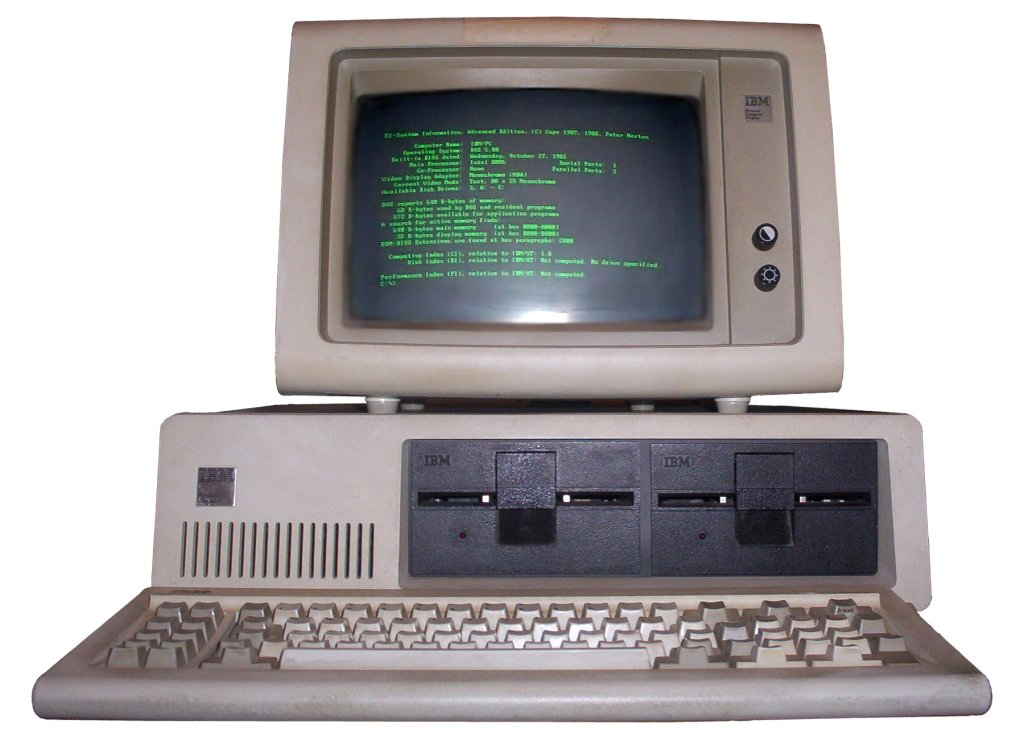
\includegraphics[width=\linewidth]{img/IBM_PC_5150.jpg}
\caption{``Зелёный'' монохромный монитор, используемый с видеоадаптером MDA}
\end{wrapfigure}

В современные видеокарты встроен графический процессор, который может выполнять дополнительную обработку данных снимая тем самым нагрузку на центральный процессор. В наши дни все современные видеокарты Nvidia и AMD (Ati) выполняют обработку графических данных на аппаратном уровне.

В 1981 году был выпущен один из самых ранних графических адаптеров в истории вычислительной техники --- MDA (Monochrome Display Adapter) для компьютеров фирмы IBM PC. Данный адаптер поддерживал только текстовый режим с разрешением $80 \times 25$ символов, помимо просто текста поддерживались текстовые атрибуты: обычный, яркий, инверсный, подчёркнутый и мигающий. Какой либо графической или цветовой информации данный адаптер обрабатывать не мог, под цветностью тогда понималось лишь свечение люминофора электронно-лучевой трубки. Последующим развитием адаптера MDA стал видеоадаптер HGC (Hercules Graphics Controller) созданный в 1982 году фирмой Hercules. Адаптер HGC поддерживал графическое разрешение $720 \times 348$ точек и две графические страницы. Поддержки цветов всё ещё не было.

Пионером в цветном изображении стала видеокарта CGA (Color Graphics Adapter) от фирмы IBM. В текстовом режиме существовало два разрешения: $40 \times 25$ символов и $80 \times 25$ символов (на каждый символ приходилась матрица $8 \times 8$ точек) с 256 символами. На каждое знакоместо приходилось 16 цветов и 16 цветов фона (либо 8 цветов фона и атрибут мигания). В графическом режиме также было два разрешения: $320 \times 200$ точек (цветность: четыре палитры по четыре цвета каждая) и $640 \times 200$ точек (данный режим был монохромным). Развитием этого адаптера стал адаптер EGA (Enhanced Graphics Adapter) с палитрой в 64 цвета. Разрешение было увеличено до $640 \times 350$. Для режима $80 \times 25$ использовалась большая матрица --- $8 \times 14$, одновременно можно было использовать 16 цветов, цветовая палитра была расширена до 64 цветов. Графический режим также позволял использовать при разрешении $640 \times 350$ 16 цветов из палитры в 64 цвета.

В ранних моделях компьютеров от IBM PS/2 использован новый графический адаптер MCGA (Multicolor Graphics Adapter). Текстовое разрешение было поднято до $640 \times 400$, что позволило использовать режим $80 \times 50$ при матрице $8 \times 8$ точек, а для режима $80 \times 25$ использовать матрицу $8 \times 16$. Количество цветов увеличено до 262144 (64 уровня яркости по каждому цвету).

\begin{wrapfigure}[12]{R}{0.5\linewidth}
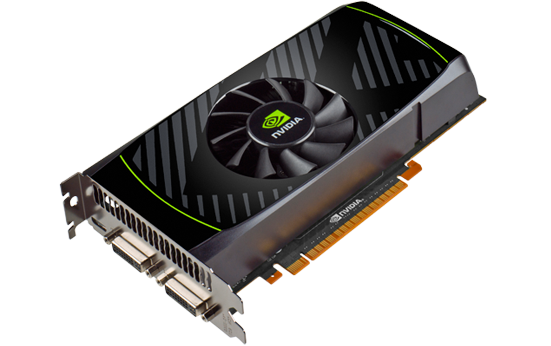
\includegraphics[width=\linewidth]{img/gtx_550_ti.png}
\caption{Видеокарта NVIDIA GTX 550 TI. 2011 год.}
\end{wrapfigure}

В 1987 году IBM создала компонентный видеоинтерфейс VGA (Video Graphics Array), улучшение графического адаптера MCGA. Добавлены: текстовое разрешение $720 \times 400$ для эмуляции MDA и графический режим $640 \times 480$.

В 1991 году появилось SVGA (Super VGA) --- расширение VGA с более высокими режимами и дополнительными возможностями, например, задание произвольной частоты кадров. Число цветов стало равно 65536 (High Color, 16 bit) и 16777216 (True Color, 24 bit).


\subsection{Устройство видеокарты}

\subsubsection{Графический процессор}

Графический процессор (Graphics processing unit (GPU) — графическое процессорное устройство) занимается расчётами выводимого изображения, освобождая от этой обязанности центральный процессор, производит расчёты для обработки команд трёхмерной графики. Является основой графической платы, именно от него зависят быстродействие и возможности всего устройства. Современные графические процессоры по сложности мало чем уступают центральному процессору компьютера, и зачастую превосходят его как по числу транзисторов, так и по вычислительной мощности, благодаря большому числу универсальных вычислительных блоков.

\begin{figure}[ht!]
\begin{center}
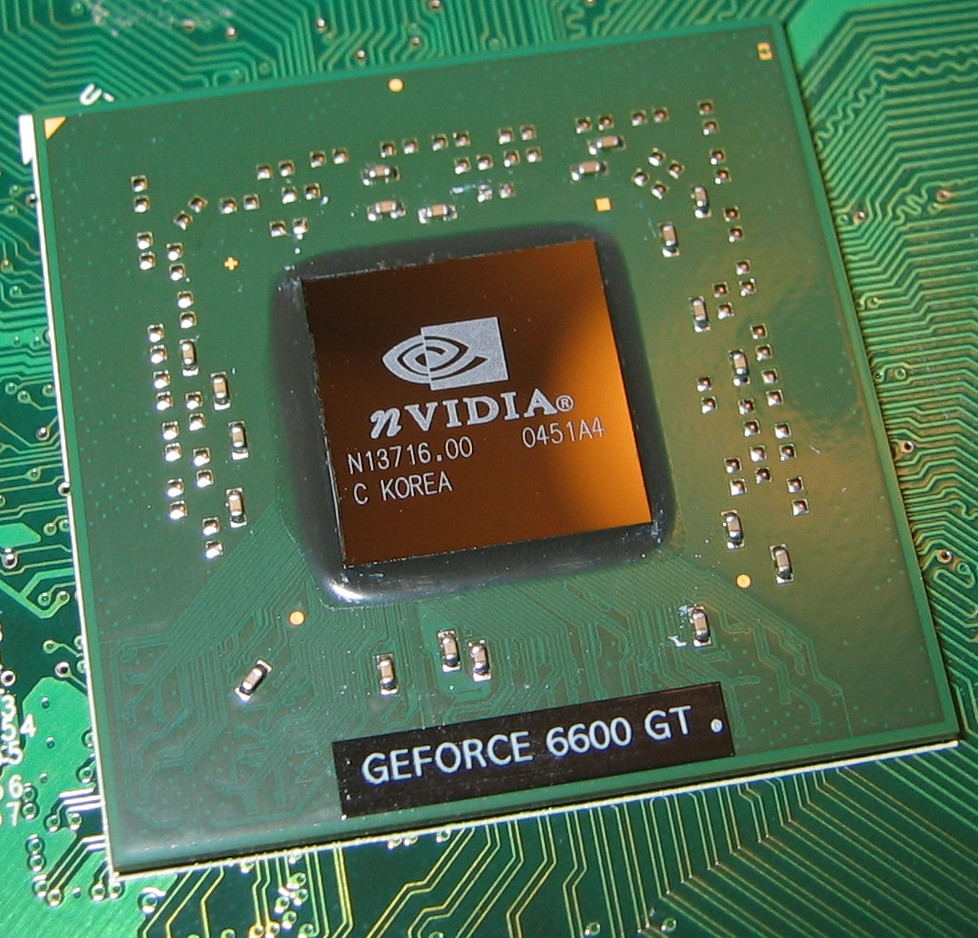
\includegraphics[width=0.3\linewidth]{img/6600GT_GPU.jpg}
\caption{Графический процессор GeForce 6600GT (NV43)}
\end{center}
\end{figure}

\subsubsection{Видеоконтроллер}

Видеоконтроллер отвечает за формирование изображения в видеопамяти и осуществляет обработку запросов центрального процессора. Современные графические адаптеры (AMD, Nvidia) обычно имеют не менее двух видеоконтроллеров, работающих независимо друг от друга и управляющих одновременно одним или несколькими дисплеями каждый.

\subsubsection{Видео-ПЗУ}

Видео-ПЗУ (Video ROM) — постоянное запоминающее устройство (ПЗУ), в которое записаны BIOS видеокарты, экранные шрифты, служебные таблицы и т. п. ПЗУ не используется видеоконтроллером напрямую — к нему обращается только центральный процессор.

\subsubsection{Видео-ОЗУ}

Видеопамять выполняет функцию кадрового буфера, в котором хранится изображение, генерируемое и постоянно изменяемое графическим процессором и выводимое на экран монитора (или нескольких мониторов). В видеопамяти хранятся также промежуточные невидимые на экране элементы изображения и другие данные. Видеопамять бывает нескольких типов, различающихся по скорости доступа и рабочей частоте.

При написании истории использовался материал \cite{hist1}.

        \section {Вычисления на графических процессорах}

В немалой степени развитию параллельных вычислений на графических процессорах способствовали компьютерные игры. Устройства для параллельных векторных вычислений, которые часто применяются в 3D графике, достигают очень высокой производительности, недоступной для универсальных процессоров. Вслед за первыми видеокартами с поддержкой параллельных вычислений возникли технологии неграфических расчётов общего назначения GPGPU (General Purpose computation on GPUs). Современные видеочипы содержат сотни математических исполнительных блоков, и эта мощь может использоваться для значительного ускорения множества вычислительно-интенсивных приложений. Разработчики задумали сделать так, чтобы GPU рассчитывали не только изображение в 3D приложениях, но и применялись в других параллельных расчётах.

В дальнейшем, два основных производителя видеочипов, AMD и Nvi\-dia, разработали и анонсировали соответствующие платформы под названием CUDA (Compute Unified Device Architecture) и AMD FireStream соответственно. В отличие от предыдущих моделей программирования GPU, эти были выполнены с учётом прямого доступа к аппаратным возможностям видеокарт. Платформы не совместимы между собой. Зато обе платформы ликвидировали некоторые из важных ограничений предыдущих моделей GPGPU, использующих традиционный графический конвейер и соответствующие Direct3D или OpenGL интерфейсы.

\subsection {Разница между CPU и GPU в параллельных расчётах}

Быстрый рост повышения частоты и производительности универсальных процессоров упёрся в физические ограничения и высокое энергопотребление, и увеличение их производительности всё чаще происходит за счёт размещения нескольких ядер в одном чипе. В универсальных процессорах каждое ядро работает отдельно от остальных, исполняя различные инструкции для различных процессов.

В видеочипах Nvidia основной блок — это мультипроцессор с восемью-десятью ядрами и сотнями ALU в целом, несколькими тысячами регистров и небольшим количеством разделяемой общей памяти. Кроме того, видеокарта содержит быструю глобальную память с доступом к ней всех мультипроцессоров, локальную память в каждом мультипроцессоре, а также специальную память для констант.

Самое главное — эти несколько ядер мультипроцессора в GPU являются SIMD (одиночный поток команд, множество потоков данных) ядрами. И эти ядра исполняют одни и те же инструкции одновременно, такой стиль программирования является обычным для графических алгоритмов и многих научных задач, но требует специфического программирования. Зато такой подход позволяет увеличить количество исполнительных блоков за счёт их упрощения.

Подытожим основные различия между строением CPU и GPU. CPU созданы для исполнения одного потока последовательных инструкций с максимальной производительностью, а GPU проектируются для быстрого исполнения большого числа параллельно выполняемых потоков инструкций. Универсальные процессоры оптимизированы для достижения высокой производительности единственного потока команд, обрабатывающего и целые числа и числа с плавающей точкой. При этом доступ к памяти случайный. 

У видеочипов работа простая и распараллеленная изначально. Видеочип принимает на входе группу полигонов, проводит все необходимые операции, и на выходе выдаёт пиксели. Обработка полигонов и пикселей независима, их можно обрабатывать параллельно, отдельно друг от друга. Поэтому, из-за изначально параллельной организации работы в GPU используется большое количество исполнительных блоков, которые легко загрузить, в отличие от последовательного потока инструкций для CPU. Кроме того, современные GPU также могут исполнять больше одной инструкции за такт (dual issue).

Как Nvidia, так и ATI поддерживают реализацию быстрого вычисления основных математических функций за один такт. К основным математическим функциям относятся: квадратный корень, экспонента, логарифм, синус, косинус и ряд других функций.

Есть различия в работе с памятью у GPU и CPU. Так, не все центральные процессоры имеют встроенные контроллеры памяти, а у всех GPU обычно есть по несколько контроллеров, вплоть до восьми 64-битных каналов в чипе Nvidia GT200. Кроме того, на видеокартах применяется более быстрая память, и в результате видеочипам доступна в разы большая пропускная способность памяти, что также весьма важно для параллельных расчётов, оперирующих с огромными потоками данных.

В универсальных процессорах большие количества транзисторов и площадь чипа идут на буферы команд, аппаратное предсказание ветвления и огромные объёмы начиповой кэш-памяти. Все эти аппаратные блоки нужны для ускорения исполнения немногочисленных потоков команд. Видеочипы тратят транзисторы на массивы исполнительных блоков, управляющие потоками блоки, разделяемую память небольшого объёма и контроллеры памяти на несколько каналов. Вышеперечисленное не ускоряет выполнение отдельных потоков, оно позволяет чипу обрабатывать нескольких тысяч потоков, одновременно исполняющихся чипом и требующих высокой пропускной способности памяти. Возможность работы с тысячами потоков накладывает свои ограничения: из-за большого количества потоков становится невозможным дать ядрам большую локальную память, ведь в этом случае вся временная память видеокарты будет уходить на обслуживание ядер. Поэтому у ядер маленькое стековое пространство, а следовательно, функции, исполняемые ядрами, не могут использовать рекурсию. Эмуляция стека за счёт памяти видеокарты возможна, но ограничена небольшим количеством итераций и является нетипичной для GPU.

Есть множество различий и в поддержке многопоточности. CPU исполняет 1-2 потока вычислений на одно процессорное ядро, а видеочипы могут поддерживать до 1024 потоков на каждый мультипроцессор, которых в чипе несколько штук. И если переключение с одного потока на другой для CPU стоит сотни тактов, то GPU переключает несколько потоков за один такт.

Вкратце можно сказать, что в отличие от современных универсальных CPU, видеочипы предназначены для параллельных вычислений с большим количеством арифметических операций. И значительно большее число транзисторов GPU работает по прямому назначению — обработке массивов данных, а не управляет исполнением (flow control) немногочисленных последовательных вычислительных потоков (Рис.~\ref{ris:gpucpu}). 

\begin{figure}[ht!]
\begin{center}
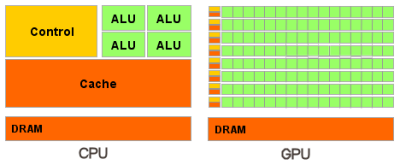
\includegraphics[width=0.8\linewidth]{img/cpu_vs_gpu.png}
\caption{Различие в устройстве CPU и GPU. DRAM --- Оперативная память, Cache --- память процессора для часто используемых операций, Control --- управляющий блок процессора, ALU --- Арифметико-логическое устройство.}
\label{ris:gpucpu}
\end{center}
\end{figure}

Параллельные вычисления на GPU начали активно развиваться с появлением шейдеров --- специальных программ предназначенных для работы на GPU. Тогда же появился компилятор языка Brook --- BrookGPU. BrookGPU облегчал программистам работу с шейдерами. Компилятор обрабатывал файлы с расширением .br и C++ программами давая на выходе скомпилированную программу работающую через DirectX или OpenGL.

Компании Nvidia и ATI увидели возможный потенциал BrookGPU и начали разрабатывать свои аналогичные проекты. Таким образом у Nvidia появился проект CUDA (Compute Unified Device Architecture), а у ATI --- CTM (Close-to-the-Metal) который был началом для AMD FireStream.

\subsection {Nvidia CUDA}

В основе программного интерфейса CUDA лежит расширенный язык Си. Для трансляции текста программы в исполняемые файлы используется компилятор nvcc, созданный на основе открытого компилятора Open64.

Обычная процедура работы с GPU выглядит следующим образом: блок геометрии вычисляет треугольники, блок растеризации вычисляет пиксели которые в дальнейшем будут отображены на экране (Рис.~\ref{ris:process}).

\begin{figure}[ht!]
\begin{center}
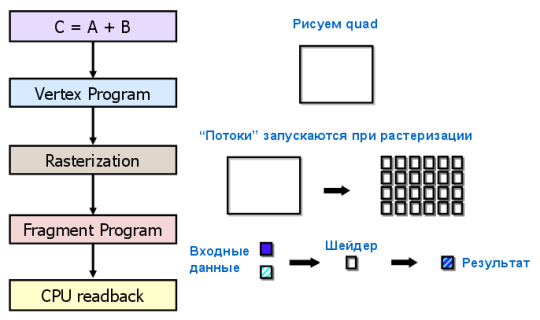
\includegraphics[width=0.5\linewidth]{img/pipeline2.png}
\caption{Обычная процедура обработки фигуры в видеокарте}
\label{ris:process}
\end{center}
\end{figure}

Поэтому использование GPGPU являлось достаточно трудоёмким процессом. Ранние методы работы с графическим процессором были нетривиальными приёмами вследствии чего были крайне неудобными. Данные представлялись изображениями (текстурами), а алгоритмы --- процессами растеризации.

CUDA представляла ряд удобств, вместо непосредственной работы с GPU:

\begin{itemize}
  \item{интерфейс программирования приложений CUDA основан на стандартном языке программирования Си с расширениями, что упрощает процесс изучения и внедрения архитектуры CUDA;}
\item{более эффективная передача данных между системной и видеопамятью;}
\item{отсутствие необходимости в графических API с избыточностью и накладными расходами;}
\item{линейная адресация памяти, и gather и scatter, возможность записи по произвольным адресам;}
\item{аппаратная поддержка целочисленных и битовых операций.}
\end{itemize}

Основные недостатки CUDA:

\begin{itemize}
\item{отсутствие поддержки рекурсии для выполняемых функций;}
\item{минимальная ширина блока в 32 потока;}
\item{закрытая архитектура CUDA, принадлежащая Nvidia.}
\end{itemize}

При написании использовался материал из \cite{nvidiacuda}.

\subsection{AMD FireStream}

Хотя цели видеокарт что у ATI, что у Nvidia одни и те же, но подходы к внутренней архитектуре всё же различаются. В первую очередь это касается основной вычислительной единицы: у Nvidia блок вычисления называется ``warp'' и состоит из 32-х нитей, у ATI блок называется ``wave front'' и состоит из 64-х нитей. Но данное различие не принципиально, практически любую программу для вычисления на GPU можно переписать для использования другого количества нитей. Конечно, может наблюдаться либо падение, либо увеличение производительности, но программа всё же будет работать.

Одно из важных отличий AMD --- это применение технологии ``VLIW'' --- Very Long Instruction Word (Рис.~\ref{ris:ati}). В графических процессорах Nvidia используются простые скалярные инструкции для работы со скалярными регистрами. В архитектуре ATI задействованы 128 битные векторные регистры. Условно назовём компоненты регистра $A$ как $a_1$, $a_2$, $a_3$ и $a_4$; а у регистра $B$ как $b_1$, $b_2$, $b_3$ и $b_4$. Тогда за один такт оказывается возможным вычислить число $a_1 \times b_1 + a_2 \times b_2 + a_3 \times b_3 + a_4 \times b_4$ или двумерный вектор $(a_1 \times b_1 + a_2 \times b_2, a_3 \times b_3 + a_4 \times b_4)$.

Производительность операций на видеокартах ATI при работе над числами одинарной точности достигает нескольких терафлопов благодаря векторным инструкциям.

Также один векторный регистр можно использовать для хранения одного числа двойной точности --- double. В этом случае можно сложить два double числа или умножить два числа, или умножить два числа и сложить с третьим за одну инструкцию. Отсюда при работе над double скорость падает в пять раз чем по сравнению с float. 

\begin{figure}[ht!]
\begin{center}
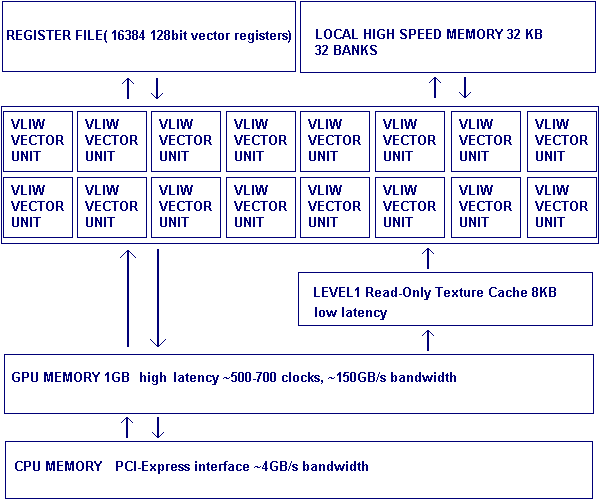
\includegraphics[width=0.8\linewidth]{img/radeon1.png}
\caption{Условная схема работы видеокарт ATI. На рисунке только один минипроцессор из нескольких параллельно работающих.}
\label{ris:ati}
\end{center}
\end{figure}

Ещё одним отличием подхода ATI от Nvidia является использование особого формата расположения инструкций в двоичной коде программы (Табл.~\ref{table:instructions}). У ATI инструкции расположены не традиционно (по тексту исходного кода программы), а секционно.

Прежде всего идёт секция с набором инструкций условных переходов, в них содержатся ссылки на секции арифметических инструкций не содержащих переходов. В секциях с арифметическими операциями (VLIW bundles --- связки VLIW-инструкций) содержатся только арифметические инструкции над данными из регистров и/или локальной памяти. Таким образом становится проще управлять потоком инструкций и доставлять их к устройствам-исполнителям. Кроме того имеются секции для инструкций обращения к памяти.

\begin{table}
\begin{center}
\begin{tabular}{|c|c|c|c|c|}
\hline
\multicolumn{5}{|c|}{Секции инструкций условных переходов} \\
\hline
Секция 0 & Ветвление 0 & \multicolumn{3}{|p{7cm}|}{Ссылка на секцию 3 непрерывных арифметических инструкций} \\ \hline
Секция 1 & Ветвление 1 & \multicolumn{3}{|p{7cm}|}{Ссылка на секцию 4} \\ \hline
Секция 2 & Ветвление 2 & \multicolumn{3}{|p{7cm}|}{Ссылка на секцию 5} \\ \hline
\multicolumn{5}{|c|}{Секции непрерывных арифметических инструкций} \\ \hline
Секция 3 & VLIW 0 & VLIW 1 & VLIW 2 & VLIW 3 \\ \hline
Секция 4 & VLIW 4 & VLIW 5 & & \\ \hline
Секция 5 & VLIW 6 & VLIW 7 & VLIW 8 & VLIW 9 \\ \hline
\end{tabular}
\end{center}
\caption {Схема разбивки программы в архитектуре видеокарт ATI}
\label{table:instructions}
\end{table}

Также существует различие в кэше L1-L2 для видеокарт Nvidia и ATI. Размеры кэша в среднем одинаковы, но существенно различаются время доступа к данным. Задержка доступа к данным у Nvidia несколько больше, и текстурные кэши позволяют сократить загрузку шины памяти, но не ускоряют доступ. У ATI задержка текстурного кэша меньше, но выше задержка локальной памяти минипроцессоров. Для быстрого перемножения матриц у Nvidia лучше использовать локальную память и загружать матрицу поблочно, в случае с AMD лучше использовать быстрый текстурный кэш и читать элементы матрицы по мере необходимости.

Для тех видов задач, которые подходят под идеологию GPU, в частности задачи векторной природы (например, умножение матриц), видеокарты AMD показывают близкую к теоретической производительность. Особенно на задачах с одинарной точностью.

Поэтому архитектура AMD более подходит для научных, профессиональных задач. Для полностью векторных задач, например в задаче параллельного подбора ключей видеокарты AMD в несколько раз опережают Nvidia и в несколько десятков раз быстрее CPU.

В целом идея AMD в том, что графический процессор должен дополнять центральный процессор компьютера выступая в роли своеобразного параллельного сопроцессора для векторных задач.

При написании раздела использовался материал из \cite{amd}.

        \section{Краткое сравнение видеокарт AMD и Nvidia}

В этом сравнении будут представлены некоторые ключевые особенности графических процессоро AMD и Nvidia (Табл.~\ref{table:compare}). Следует, однако, учитывать что это сравнение носит примерный характер. Между фирмами AMD и Nvidia всегда идёт борьба за рынок поэтому нет ничего удивительного что внутренняя архитектура может меняться от модели к модели.

\begin{table}
\begin{center}
\begin{tabular}{|p{5cm}|p{5cm}|}
\hline
AMD & Nvidia \\ \hline
Технология FireStream & CUDA \\ \hline
64 нити в блоке & 32 нити в блоке \\ \hline
Использование секций с данными & Традиционное построение программ \\ \hline
Меньше возможности для рекурсии & Больше возможностей для рекурсии \\ \hline
Теоретически более быстрая производительность & Меньшая производительность \\ 
\hline
\end{tabular}
\end{center}
\caption{Краткое сравнение графических процессоров AMD и Nvidia}
\label{table:compare}
\end{table}

При написании использовался материал из \cite{nvidiacuda} и \cite{amd}.

        \section{Применение параллельных вычислений}

Сегодня параллельные вычисления с применением графических процессоров используются во многих сферах начиная с медицинской науки и заканичивая, но не ограничиваясь прогнозированием погоды. Ниже представлены некоторые области применения графических ускорителей.

\begin{itemize}
\item{Медицина}
  \begin{itemize}
  \item{В Австралийском национальном университете проводятся исследования развития болезни Паркинсона с помощью методов машинного обучения\cite{almanac1}.}
  \item{В стартапе Zebra Medical Vision накопленные данные в клинических исследованиях используются для оценки рисков развития болезней, их предупреждения и помощи в организации и проведении профилактических лечений\cite{almanac1}.}
  \item{В нью-йоркской Школе медицины Икана при больнице Маунт-Синай глубокое обучение используется для анализа медицинских карт и определения пациентов, с высоким риском заболевания опасными болезнями в течении года\cite{almanac2}.}
 \end{itemize}

\item{Энергетика}

\begin{itemize}
  \item{Компания-стартап PowerScout из Калифорнии применяет GPU для прогнозирования, какие домохозяйства могут с большой долей вероятности приобрести солнечные панели. Разработки \selectlanguage{english}{Po\-wer\-Scout} также позволяют определить объём энергии, который можно получить с крыши одного дома. При этом необязательно самостоятельно проводить подсчёты. Необходимые данные извлекаются из коммерческих баз, спутниковых снимков. Также учитываются возможные затенения, например деревья рядом с домами, отбрасывающие тень на крыши\cite{almanac1}.}  
\end{itemize}

\item{Астрономия}

\begin{itemize}
  \item{В Университетском колледже Лондона вычисления на GPU используются для определения планет, на которых возможно поддерживать жизнь. Название программы --- RobERt (Ro\-bo\-tic Exo\-pla\-net Re\-co\-gni\-tion, ``роботизированное распознавание эк\-зо\-пла\-нет'')\cite{almanac2}.}
\end{itemize}

\item{Агрономия}

\begin{itemize}
\item{Немецкая компания PEAT применяет глубокое обучение для создания инструмента для диагностики и лечения болезней растений. Пользователь фотографирует больные растения и загружает полученные изображения в программу PEAT ``Plantix'', после чего получает рекомендации по лечению\cite{almanac3}.}
\end{itemize}

\item{Химия}

\begin{itemize}
\item{Abalone --- программа молекулярного моделирования, предназначенная для изучения молекулярной динамики био\-по\-ли\-ме\-ров\cite{chem}\footnote{\url{http://www.biomolecular-modeling.com/Abalone/}}.}

\item{CP2K --- программа для атомарной и молекулярной симуляции твёрдых тел, жидкостей, молекулярных и биологических сис\-тем\cite{chem}\footnote{\url{https://www.cp2k.org/}}.}


\end{itemize}
\end{itemize}

        \section{Заключение}

Ключевым фактором, определяющим сегодня развитие ИИ-технологий, считается темп роста вычислительной мощности компьютеров, так как принципы работы человеческой психики по-прежнему остаются неясными (на доступном для моделирования уровне детализации). Поэтому тематика ИИ-конференций выглядит достаточно стандартно и по составу почти не меняется уже довольно давно.

Но рост производительности современных компьютеров в сочетании с повышением качества алгоритмов периодически делает возможным применение различных научных методов на практике. Так случилось с интеллектуальными игрушками, так происходит с домашними роботами. Снова будут интенсивно развиваться временно забытые методы простого перебора вариантов (как в шахматных программах), обходящиеся крайне упрощенным описанием объектов. Но с помощью такого подхода (главный ресурс для его успешного применения --- производительность) удастся решить, как ожидается, множество самых разных задач (например, из области криптографии). Уверенно действовать автономным устройствам в сложном мире помогут достаточно простые, но ресурсоемкие алгоритмы адаптивного поведения. При этом ставится цель разрабатывать системы, не внешне похожие на человека, а действующие, как человек.

Ученые пытаются заглянуть и в более отдаленное будущее. Можно ли создать автономные устройства, способные при необходимости самостоятельно собирать себе подобные копии (размножаться)? Способна ли наука создать соответствующие алгоритмы? Сможем ли мы контролировать такие машины? Ответов на эти вопросы пока нет. Продолжится активное внедрение формальной логики в прикладные системы представления и обработки знаний. В то же время такая логика не способна полноценно отразить реальную жизнь, и произойдет интеграция различных систем логического вывода в единых оболочках. При этом, возможно, удастся перейти от концепции детального представления информации об объектах и приемов манипулирования этой информацией к более абстрактным формальным описаниям и применению универсальных механизмов вывода, а сами объекты будут характеризоваться небольшим массивом данных, основанных на вероятностных распределениях характеристик.

Сфера ИИ, ставшая зрелой наукой, развивается постепенно --- медленно, но неуклонно продвигаясь вперед. Поэтому результаты достаточно хорошо прогнозируемы, хотя на этом пути не исключены и внезапные прорывы, связанные со стратегическими инициативами. 

        \Csection{Литература}

В процессе написания курсовой работы использовалась следующая литература:

\begin{enumerate}
\item{Лекции по теории систем. Коган Д.И.}
\item{Структура и интерпретация компьютерных программ. Харольд Абельсон, Джеральд Джей Сассман, Джули Сассман. Добросвет. 2006.}
\end{enumerate}

%        \input{src/CG/amdgpu.tex}
%        \Csection{Текст программы}

\begin{lstlisting}[style=customoz, caption=widget.h]
#ifndef WIDGET_H
#define WIDGET_H

#include <QWidget>
#include <QPainter>
#include <math.h>
#include <QPushButton>
#include <QVBoxLayout>
#include <QGroupBox>
#include <QSlider>
#include <QLabel>
#include "Object3D.h"
#include "Autopilot.h"
#include <QComboBox>

// Основной класс
class Widget : public QWidget
{
    Q_OBJECT
private:
    // Слайдер поворота вокруг оси Z
    QSlider * aroundZSlider;
    QLabel * zAngleLabel;

    // Слайдер поворота вокруг оси X
    QSlider * aroundXSlider;
    QLabel * xAngleLabel;

    // Слайдер поворота вокруг оси Y
    QSlider * aroundYSlider;
    QLabel * yAngleLabel;

    // Трёхмерный объект
    Object3D * object3d;

    // Клавиша запуска автопилота
    QPushButton * autoPilotButton;

    // Объект автопилота
    Autopilot * myAutopilot;

    // Тред для автопилота
    QThread * myThread;

    // Отображение включённости автопилота
    bool autopilotIsEnabled;

    // ComboBox с трёхмерными фигурами
    QComboBox * shapeComboBox;

    // Процедура установки нового объекта
    void setNewObject();
public:
    Widget(QWidget *parent = 0);
    void paintEvent(QPaintEvent *);
    ~Widget();
public  slots:

    // Реакция на изменение слайдера с углом Z
    void sliderZchanged(int value);

    // Реакция на изменение слайдера с углом X
    void sliderXchanged(int value);

    // Реакция на изменение слайдера с углом Y
    void sliderYchanged(int value);

    // Реакция на нажатие клавиши автопилота
    void buttonAutopilotPressed();

    // Реакция на сигнал с новыми углами поворотов от автопилота
    void autopilotDatas(qreal XAngle,
                        qreal YAngle,
                        qreal ZAngle);

    // Реакция на выбор фигуры из ComboBox-а
    void selectShape();

    // Реакция на паузу автопилота
    void autopilotPaused();
};

#endif // WIDGET_H
\end{lstlisting}

\begin{lstlisting}[style=customoz, caption=widget.cpp]
#include "widget.h"

// Конструктор главного объекта
Widget::Widget(QWidget *parent)
    : QWidget(parent)
{
    this->setStyleSheet("background: black;");
    autopilotIsEnabled = false;
    QGroupBox * controlPanel = new QGroupBox(tr("Control panel"));
    QVBoxLayout * controlPanelLayout = new QVBoxLayout;

    // Слайдер для вращения вокруг оси Z
    aroundZSlider = new QSlider(Qt::Horizontal, controlPanel);
    aroundZSlider->setMinimum(0);
    aroundZSlider->setMaximum(360);
    aroundZSlider->setValue(0);
    zAngleLabel = new QLabel("Z angle: " +
                             QString::number(aroundZSlider->value()),
                             controlPanel);
    connect(aroundZSlider, SIGNAL(valueChanged(int)), this,
            SLOT(sliderZchanged(int)));

    // Слайдер для вращения вокруг оси X
    aroundXSlider = new QSlider(Qt::Horizontal, controlPanel);
    aroundXSlider->setMinimum(0);
    aroundXSlider->setMaximum(360);
    aroundXSlider->setValue(0);
    xAngleLabel = new QLabel("X angle: " + QString::number(aroundXSlider->value()),
                             controlPanel);
    connect(aroundXSlider, SIGNAL(valueChanged(int)), this,
            SLOT(sliderXchanged(int)));

    // Слайдер для вращения вокруг оси Y
    aroundYSlider = new QSlider(Qt::Horizontal, controlPanel);
    aroundYSlider->setMinimum(0);
    aroundYSlider->setMaximum(360);
    aroundYSlider->setValue(0);
    yAngleLabel = new QLabel("Y angle: " + QString::number(aroundYSlider->value()),
                             controlPanel);
    connect(aroundYSlider, SIGNAL(valueChanged(int)), this,
            SLOT(sliderYchanged(int)));

    // Клавиша автопилота
    autoPilotButton = new QPushButton("Enable autopilot", controlPanel);
    connect(autoPilotButton, SIGNAL(clicked()), SLOT(buttonAutopilotPressed()));

    // Задание выпадающего списка с фигурами
    shapeComboBox = new QComboBox;
    shapeComboBox->addItem("Cube");
    shapeComboBox->addItem("Pyramid");
    shapeComboBox->addItem("Star");
    connect(shapeComboBox, SIGNAL(currentIndexChanged(int)), SLOT(selectShape()));

    // Задание фигуры
    qreal cubeDots[8][3] = {{50, -50, -50}, {50, -50, 50},
                            {50, 50, 50}, {50, 50, -50},
                            {-50, -50, -50}, {-50, -50, 50},
                            {-50, 50, 50}, {-50, 50, -50}};
    int cubeLinks[] = {0, 1, 0, 4, 0, 3, 1, 2, 1, 5, 2, 6, 2, 3, 3, 7, 5, 6, 5, 4,
                       6, 7, 4, 7};
    object3d = new Object3D(&cubeDots[0][0], 8, &cubeLinks[0], 24);

    // Добавление виджетов на слой компоновки
    controlPanelLayout->addWidget(zAngleLabel);
    controlPanelLayout->addWidget(aroundZSlider);

    controlPanelLayout->addWidget(xAngleLabel);
    controlPanelLayout->addWidget(aroundXSlider);

    controlPanelLayout->addWidget(yAngleLabel);
    controlPanelLayout->addWidget(aroundYSlider);

    controlPanelLayout->addWidget(autoPilotButton);

    controlPanelLayout->addWidget(shapeComboBox);
    controlPanel->setLayout(controlPanelLayout);
    controlPanel->show();
}

void Widget::buttonAutopilotPressed(){
    // Реакция на нажатие клавиши автопилота
    if (autopilotIsEnabled) {
        // Если автопилот уже был запущен
        myAutopilot->stop();
        aroundXSlider->setEnabled(true);
        aroundYSlider->setEnabled(true);
        aroundZSlider->setEnabled(true);
        autoPilotButton->setText("Enable autopilot");
        autopilotIsEnabled = false;
    }
    else {
        // Если автопилот не был запущен
        myThread = new QThread;
        myAutopilot = new Autopilot(object3d->getAngleX(),
                                    object3d->getAngleY(),
                                    object3d->getAngleZ());
        myAutopilot->moveToThread(myThread);
        connect(myAutopilot, SIGNAL(newAngles(qreal,qreal,qreal)),
                SLOT(autopilotDatas(qreal,qreal,qreal)));
        connect(myAutopilot, SIGNAL(pausedSignal()),
                SLOT(autopilotPaused()));
        connect(myThread, SIGNAL(started()), myAutopilot,
                SLOT(start()));
        connect(myAutopilot, SIGNAL(finished()), myThread,
                SLOT(quit()));
        connect(myAutopilot, SIGNAL(finished()), myAutopilot,
                SLOT(deleteLater()));
        connect(myThread, SIGNAL(finished()), myThread,
                SLOT(deleteLater()));
        aroundXSlider->setEnabled(false);
        aroundYSlider->setEnabled(false);
        aroundZSlider->setEnabled(false);

        // Смена раскраски слайдеров
        QPalette disablePalette = aroundXSlider->palette();
        disablePalette.setColor(QPalette::Disabled,
                                QPalette::Light,
                                QColor(128, 128, 128));
        aroundXSlider->setPalette(disablePalette);
        aroundYSlider->setPalette(disablePalette);
        aroundZSlider->setPalette(disablePalette);
        autoPilotButton->setText("Disable autopilot");
        myThread->start();
        autopilotIsEnabled=true;
    }
}

void Widget::paintEvent(QPaintEvent *){
    // Процедура отрисовки окна с изображением
    this->setWindowTitle("Width: " +
                         QString::number(this->width()) +
                         " Height: " +
                         QString::number(this->height()));
    QPainter painter(this);
    painter.setPen(Qt::blue);
    qreal windowHalfHeight = this->height()/2,
            windowHalfWidth = this->width()/2;
    int firstDot, secondDot;

    // Отрисовка трёхмерного объекта
    for (int i = 0; i < object3d->getLinksCount(); i++){
        firstDot = object3d->getLinkFirstDot(i);
        secondDot = object3d->getLinkSecondDot(i);
        painter.drawLine(QPoint(object3d->getY(firstDot) +
                                windowHalfWidth,
                                object3d->getX(firstDot) +
                                windowHalfHeight),
                         QPoint(object3d->getY(secondDot) +
                                windowHalfWidth,
                                object3d->getX(secondDot) +
                                windowHalfHeight));
    }
}

Widget::~Widget()
{
    // Деструктор виджета
}

void Widget::sliderZchanged(int value){
    // Реакция на изменение слайдера с углом Z
    zAngleLabel->setText("Z angle: " +
                         QString::number(value));
    object3d->setZAngle(value*3.14/180);
    update();
}

void Widget::sliderXchanged(int value){
    // Реакция на изменение слайдера с углом X
    xAngleLabel->setText("X angle: " +
                         QString::number(value));
    object3d->setXAngle(value*3.14/180);
    update();
}

void Widget::sliderYchanged(int value){
    // Реакция на изменение слайдера с углом Y
    yAngleLabel->setText("Y angle: " +
                         QString::number(value));
    object3d->setYAngle(value*3.14/180);
    update();
}

void Widget::autopilotDatas(qreal XAngle, qreal YAngle, qreal ZAngle){
    // Реакция на сигнал с новыми углами поворотов от автопилота
    object3d->setXAngle(XAngle);
    object3d->setYAngle(YAngle);
    object3d->setZAngle(ZAngle);
    aroundXSlider->setValue((((int)(XAngle * 180 / 3.14) % 360)+360)%360);
    aroundYSlider->setValue((((int)(YAngle * 180 / 3.14) % 360)+360)%360);
    aroundZSlider->setValue((((int)(ZAngle * 180 / 3.14) % 360)+360)%360);
    update();
}

void Widget::selectShape(){
    // Реакция на выбор фигуры из ComboBox-а
    if (!autopilotIsEnabled){
        setNewObject();
    }
    else myAutopilot->pauseOnOff();
}

void Widget::setNewObject(){
    // Процедура установки нового объекта в myObject
    switch (shapeComboBox->currentIndex()) {
    case 0:
    {
        // Реализация трёхмерного объекта "Куб"
        qreal cubeDots[8][3] = {{50, -50, -50}, {50, -50, 50}, {50, 50, 50},
                                {50, 50, -50}, {-50, -50, -50}, {-50, -50, 50},
                                {-50, 50, 50}, {-50, 50, -50}};
        int cubeLinks[] = {0, 1, 0, 4, 0, 3, 1, 2, 1, 5, 2, 6,
                           2, 3, 3, 7, 5, 6, 5, 4, 6, 7, 4, 7};
        object3d->setObject(&cubeDots[0][0], 8, &cubeLinks[0], 24);
        update();
    }
        break;
    case 1:
    {
        // Реализация трёхмерного объекта "Пирамида"
        qreal tetraDots[4][3] = {{0, 0, 100}, {0, -100, 0}, {-50, 50, 0},
                                 {50, 50, 0}};

        int tetraLinks[] = {0, 1, 0, 2, 0, 3, 1, 0, 1, 2, 1, 3, 2, 0, 2, 1,
                            2, 3, 3, 0, 3, 1, 3, 2};
        object3d->setObject(&tetraDots[0][0], 4, &tetraLinks[0], 24);
        update();
    }
        break;
    case 2:
    {
        qreal starDots[12][3] = {{200, 0, 0}, {60, 190, 0}, {-160, 116, 0},
                                 {-160, -116, 0}, {60, -190, 0}, {60, 44, 0},
                                 {-22, 72, 0}, {-76, 0, 0}, {-22, -72, 0},
                                 {60, -44, 0}, {0, 0, 25}, {0, 0, -25}};
        int starLinks[] = {0, 5, 0, 10, 0, 11, 0, 9, 1, 5, 1, 6, 1, 11,
                          1, 10, 2, 6, 2, 7, 2, 11, 2, 10, 3, 7, 3, 8,
                          3, 11, 3, 10, 4, 8, 4, 9, 4, 11, 4, 10, 5, 11,
                          5, 10, 6, 11, 6, 10, 7, 11, 7, 10, 8, 11, 8, 10,
                          9, 11, 9, 10};
        object3d->setObject(&starDots[0][0], 12, &starLinks[0], 60);
        update();

    }
        break;
    default:
        break;
    }
}

void Widget::autopilotPaused(){
    // Смена объекта при паузе автопилота
    setNewObject();
    myAutopilot->pauseOnOff();
}
\end{lstlisting}

\begin{lstlisting}[style=customoz, caption=Object3D.h]
#ifndef OBJECT3D_H
#define OBJECT3D_H
#include <QtGlobal>
#include <cmath>

const int three = 3, two = 2, zero = 0;

// Класс трёхмерного объекта
class Object3D{
private:
    qreal ** objectDots; // Координаты (x, y, z)
    int dotsCount; // Количество точек
    int *dotsLinks; // Взаимосвязи точек (1 соединяется с 2 и т.д.)
    int linksCount; // Количество связей
    qreal angleZ; // Поворот вокруг оси Z (радианы)
    qreal angleX; // Поворот вокруг оси X (радианы)
    qreal angleY; // Поворот вокруг оси Y (радианы)
    qreal maxD; // Дистанция от начала координат то самой удалённой точки

    // Расстояние от центра до самой удалённой точки 3Д объекта
    qreal maxDistance();
    // Сброс данных (при смене фигуры), углы сохраняются
    void resetObject();

public:
    // Конструктор, dots - массив точек, r - количество точек
    // links - связи между точками, linksCount - количество связей
    Object3D(qreal *dots, int r, int * links, int totalLinksCount);

    // Возврат координаты X какой-либо точки. Отсчёт от 0.
    qreal getX(int dotNumber);

    // Возврат координаты Y какой-либо точки. Отсчёт от 0.
    qreal getY(int dotNumber);

    // Возврат координаты Z какой-либо точки. Отсчёт от 0.
    qreal getZ(int dotNumber);

    // Вернуть количество связей. Отсчёт от 1.
    int getLinksCount();

    // Вернуть количество точек. Отсчёт от 1.
    int getDotsCount();

    // Вернуть номер первой точки из связи
    int getLinkFirstDot(int linkNumber);

    // Вернуть номер второй точки из связи
    int getLinkSecondDot(int linkNumber);

    // Установить поворот вокруг оси Z (в радианах)
    void setZAngle(qreal angle);

    // Установить поворот вокруг оси X (в радианах)
    void setXAngle(qreal angle);

    // Установить поворот вокруг оси Y (в радианах)
    void setYAngle(qreal angle);

    // Возращение углов поворота вокруг осей
    qreal getAngleZ();
    qreal getAngleX();
    qreal getAngleY();

    // Возвращает максимальную дистанцию
    qreal getMaxDistance();

    // Установка нового объекта
    void setObject(qreal *, int, int *, int);
};

#endif // OBJECT3D_H
\end{lstlisting}

\begin{lstlisting}[style=customoz, caption=Object3D.cpp]
#include "Object3D.h"

Object3D::Object3D(qreal *dots, int r, int * links,
                   int totalLinksCount){
    // Конструктор объекта
    // Загружаем координаты точек объекта
    objectDots = new qreal * [r];
    dotsCount = r;
    for (int j = zero; j < r; j++){
        objectDots[j] = new qreal [three];
        for (int i = zero; i < three; i++)
            objectDots[j][i] = dots[j*three + i];
    }

    // Загружаем связи точек
    dotsLinks = new int [totalLinksCount];
    linksCount = totalLinksCount / 2;
    for (int j = zero; j < totalLinksCount; j++){
        dotsLinks[j] = links[j];
    }

    // Выставление начальных углов
    setXAngle(0);
    setYAngle(0);
    setZAngle(0);

    // Дистанция от начала координат до дальней точки
    maxD = maxDistance();
}

qreal Object3D::getX(int dotNumber){
    // Возврат координаты X какой-либо точки
    if (dotNumber <= dotsCount - 1)
        return (objectDots[dotNumber][0] * cos (angleZ) -
                objectDots[dotNumber][1] * sin(angleZ)) * cos (angleY) +
                objectDots[dotNumber][2] * sin(angleY);
    else
        return zero;
}

qreal Object3D::getY(int dotNumber){
    // Возврат координаты Y какой-либо точки
    if (dotNumber <= dotsCount - 1)
        return (objectDots[dotNumber][1] * cos(angleZ) +
                objectDots[dotNumber][0] * sin(angleZ)) * cos(angleX) -
                objectDots[dotNumber][2] * sin(angleX);
    else
        return zero;
}

qreal Object3D::getZ(int dotNumber){
    // Возврат координаты Z какой-либо точки
    if (dotNumber <= dotsCount - 1)
        return (objectDots[dotNumber][2] * cos(angleX) +
                objectDots[dotNumber][1] * sin(angleX)) * cos(angleY) -
                objectDots[dotNumber][0] * sin(angleY);
    else
        return zero;
}

int Object3D::getLinksCount(){
    // Возврат количества связей
    return linksCount;
}

int Object3D::getDotsCount(){
    // Возврат количества точек
    return dotsCount;
}

int Object3D::getLinkFirstDot(int linkNumber){
    // Возврат номера первой точки из связи
    if (linkNumber <= linksCount - 1 && linkNumber >= 0)
        return dotsLinks[linkNumber * 2];
    else
        return -1;
}

int Object3D::getLinkSecondDot(int linkNumber){
    // Возврат номера второй точки из связи
    if (linkNumber <= linksCount - 1 && linkNumber >= 0)
        return dotsLinks[linkNumber * 2 + 1];
    else
        return -1;
}

void Object3D::setZAngle(qreal angle){
    // Установка угла поворота вокруг оси Z
    angleZ = angle;
}

void Object3D::setXAngle(qreal angle){
    // Установка угла поворота вокруг оси X
    angleX = angle;
}

void Object3D::setYAngle(qreal angle){
    // Установка угла поворота вокруг оси Y
    angleY = angle;
}

qreal Object3D::maxDistance()
{
    // Вычисление дистанции от начала координат до дальней точки
    qreal distance = 0, temp;

    for (int i = 0; i < dotsCount; i++){
        temp = sqrt(getX(i)*getX(i) + getY(i)*getY(i) + getZ(i)*getZ(i));
        if (temp > distance) distance = temp;
    }
    return distance;
}

qreal Object3D::getMaxDistance()
{
    // Возврат дистанции от начала координат до дальней точки
    return maxD;
}

qreal Object3D::getAngleX(){
    // Возврат угла поворота вокруг оси X
    return angleX;}

qreal Object3D::getAngleY(){
    // Возврат угла поворота вокруг оси Y
    return angleY;}

qreal Object3D::getAngleZ(){
    // Возврат угла поворота вокруг оси Z
    return angleZ;}

void Object3D::resetObject(){
    // Сброс данных объекта
    delete [] objectDots;
    dotsCount = 0;
    delete [] dotsLinks;
    linksCount = 0;
    maxD = 0;
}

void Object3D::setObject(qreal * dots, int r, int * links, int totalLinksCount){
    // Установка нового объекта
    // Загружаем координаты точек объекта
    objectDots = new qreal * [r];
    dotsCount = r;
    for (int j = zero; j < r; j++){
        objectDots[j] = new qreal [three];
        for (int i = zero; i < three; i++)
            objectDots[j][i] = dots[j*three + i];
    }

    // Загружаем связи точек
    dotsLinks = new int [totalLinksCount];
    linksCount = totalLinksCount / 2;
    for (int j = zero; j < totalLinksCount; j++){
        dotsLinks[j] = links[j];
    }
    maxD = maxDistance();
}
\end{lstlisting}

\begin{lstlisting}[style=customoz, caption=Autopilot.h]
#ifndef AUTOPILOT_H
#define AUTOPILOT_H
#include <QObject>
#include <ctime>
#include <QThread>
#include "Sleeper.h"

// Класс автопилота
class Autopilot : public QObject{
    Q_OBJECT
private:
    qreal startXAngle, startYAngle, startZAngle; // Начальные углы по осям
    qreal vX, vY, vZ; // Скорость изменения угла в секунду
    bool enabled; // Запущен ли процесс
    bool paused; // Приостановлен ли процесс
    qreal generateSpeed(); // Генерация угловых скоростей
    qreal currentSeconds; // Текущее время от начала работы
    void process(); // Основной рабочий процесс автопилота
public:
    // Конструктор
    Autopilot(qreal XAngle, qreal YAngle, qreal ZAngle);

    // Деструктор
    ~Autopilot();

public slots:
    // Слот запуска процесса
    void start();

    // Слот останова процесса
    void stop();

    // Слот паузы вкл/выкл
    void pauseOnOff();
signals:

    // Сигнал с новыми углами
    void newAngles(qreal XAngle, qreal YAngle, qreal ZAngle);

    // Сигнал завершения работы автопилота
    void finished();

    // Сигнал о вставании на паузу
    void pausedSignal();
};
#endif // AUTOPILOT_H
\end{lstlisting}

\begin{lstlisting}[style=customoz, caption=Autopilot.cpp]
#include "Autopilot.h"

Autopilot::Autopilot(qreal XAngle,
                     qreal YAngle,
                     qreal ZAngle){
    // Конструктор автопилота
    std::srand(std::time(0) * 29);
    startXAngle = XAngle;
    startYAngle = YAngle;
    startZAngle = ZAngle;
    vX = generateSpeed();
    vY = generateSpeed();
    vZ = generateSpeed();
    currentSeconds = 0;
    enabled = false;
    paused = false;
}

Autopilot::~Autopilot(){
    // Деструктор автопилота
}

qreal Autopilot::generateSpeed(){
    // Генерация новой скорости
    return std::rand() * 3.14 / RAND_MAX-1.57;
}

void Autopilot::start(){
    // Запуск автопилота
    enabled = true;
    process();
}

void Autopilot::stop(){
    // Останов автопилота
    enabled = false;
}

void Autopilot::pauseOnOff(){
    // Пауза автопилота вкл/выкл
    if (paused) paused = false;
    else {
        paused = true;
        emit pausedSignal();
    }
}

void Autopilot::process(){
    // Основной процесс автопилота
    while (enabled){
        if (!paused){
            Sleeper::msleep(100);
            currentSeconds += 0.1;
            emit newAngles(vX*currentSeconds + startXAngle,
                           vY*currentSeconds + startYAngle,
                           vZ*currentSeconds + startZAngle);}
        else Sleeper::msleep(100);
    }
    emit finished();
}
\end{lstlisting}

\begin{lstlisting}[style=customoz, caption=Sleeper.h]
#ifndef SLEEPER_H
#define SLEEPER_H
#include <QThread>

// Объект паузы в процессе работы треда
class Sleeper : public QThread
{
public:
    static void usleep(unsigned long usecs){QThread::usleep(usecs);}
    static void msleep(unsigned long msecs){QThread::msleep(msecs);}
    static void sleep(unsigned long secs){QThread::sleep(secs);}
};
#endif // SLEEPER_H
\end{lstlisting}

\begin{lstlisting}[style=customoz, caption=main.cpp]
#include "widget.h"
#include "Object3D.h"
#include <QApplication>

int main(int argc, char *argv[])
{
    QApplication a(argc, argv);

    Widget w;
    w.show();
    return a.exec();
}
\end{lstlisting}

%	\section{Задание 1}

Создайте объект, в котором блоковый элемент размерами 250 на 250 и заливкой красного цвета заключён в рамку тёмно-синего цвета типа inset и толщиной 10. По нажатию кнопки изменять цвет заливки на голубой и надпись на кнопке. При следующем нажатии изменять цвет заливки на красный и надпись на кнопке.

\begin{center}
  \includegraphics{img/Exercise_01/01.png}
  \includegraphics{img/Exercise_01/02.png}
  \includegraphics{img/Exercise_01/03.png}
\end{center}

Исходный код \verb|exercise_01.html|:

\begin{verbatim}
<!DOCTYPE HTML>
<html>
  <head>
    <meta charset="utf-8">
    <title>Смена цвета</title>
    <style type="text/css">
      .block1 {
      width: 250px;
      height: 250px;
      background: red;
      padding: 5px;
      padding-right: 20px;
      border: inset 10px #0b0b3b;
      float: left;
      }
      
      .block2 {
          width: 100%;
          height: auto;
	  float: left;
      }
    </style>
    <script>
      function changeColorLabel(){
	  var myButton=document.getElementById('button');
	  var myDiv=document.getElementById('changedDiv');
	  if (myButton.value=="изменить фон на синий"){
	      myButton.value="изменить фон на красный";
	      myDiv.style.background="blue";
	  }
	  else{
	      myButton.value="изменить фон на синий";
	      myDiv.style.background="red";}
      }
    </script>
  </head>
  <body>
      <div class="block1" id='changedDiv'></div>
      <div class="block2"><input type="button"
				 id='button'
				 onClick="changeColorLabel();"
				 value="изменить фон на синий"/></div>
  </body>
</html>
\end{verbatim}

 %       \section{Задание 2}

Сначала на странице две картинки в рамках и две кнопки с надписью ``Спрячь меня''. При нажатии на кнопку картинка прячется, и надпись на кнопке меняется на ``Покажи меня''. Если ещё раз нажать на кнопку, картинка появляется и меняется надпись на кнопке.

При нажатии на кнопку ``[Следующая картинка]'':

\begin{center}
  \includegraphics[width=10cm]{img/Exercise_02/01.png}
  \includegraphics[width=10cm]{img/Exercise_02/02.png}
  \includegraphics[width=10cm]{img/Exercise_02/03.png}
  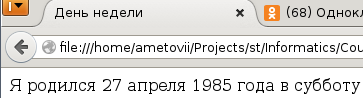
\includegraphics[width=10cm]{img/Exercise_02/04.png}
  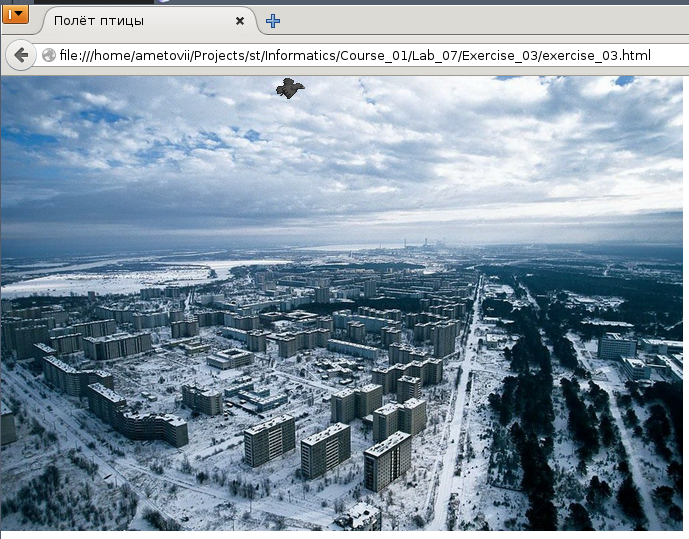
\includegraphics[width=10cm]{img/Exercise_02/05.png}
\end{center}

Исходный код \verb|exercise_02.html|:


\begin{verbatim}
<!DOCTYPE HTML>
<html>
  <head>
    <meta charset="utf-8">
    <title>Работа с отображениями картинок</title>
    <style type="text/css">
      body {
      background: darkblue;
      }
      .block1 {
          width: auto;
          height: auto;
	  float: left;
          border: outset 50px #ffA089;
      }
      
      .block2 {
          width: auto;
          height: auto;
	  float: left;
          border: outset 50px #89ffA0;
      }
    </style>
    <script>
      function changeVisibility(imageNumber){
	  var someImage=document.getElementById(imageNumber);
	  var someButton=document.getElementById('button'+
						 imageNumber);
	  if (someImage.style.display=='none'){
	      someImage.style.display='block';
	      someButton.value="Спрячь меня";
	  }
	  else {
	      someImage.style.display='none';
	      someButton.value="Покажи меня";
	  }
      }
    </script>
  </head>
  <body>
    <table cellspacing="0" cellpadding="0">
      <tr>
	<td>
	  <div class="block1" id='1'>
	    <img style="margin: 5px;" src="Pictures/01.jpeg">
	  </div>
	</td>
	<td>
	  <div class="block2" id='2'>
	    <img style="margin: 5px;" src="Pictures/02.jpg">
	  </div>
	</td>
      </tr>
      <tr>
	<td>
	  <input type="button"
		 style="width: 100%;"
		 value="Спрячь меня" id='button1'
		 onClick="changeVisibility(1)"/>
	</td>
	<td>
	  <input type="button"
		 style="width: 100%;"
		 value="Спрячь меня" id='button2'
		 onClick="changeVisibility(2)"/>
	</td>
      </tr>
    </table>
  </body>
</html>
\end{verbatim}

  %      \section{Задание 3 --- обмен информацией с Web-сервером}

Создайте веб-приложение, которое формирует возрастающую последовательность из чисел, переданных через поля ввода формы.

Ввод данных:

\begin{center}
  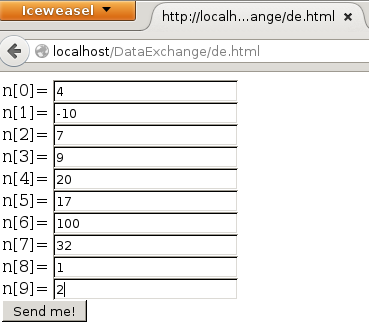
\includegraphics[width=9cm]{img/09.png}
\end{center}

Результат:

\begin{center}
  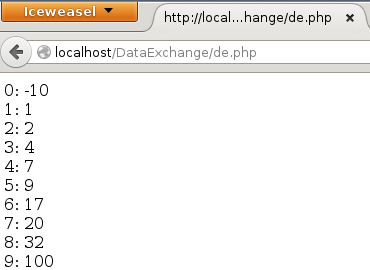
\includegraphics[width=9cm]{img/10.png}
\end{center}

Исходный код \verb|de.html|:

\begin{verbatim}
<form action="de.php" method="post">
  n[0]=  <input type="text" name="n0" /><br />
  n[1]=  <input type="text" name="n1" /><br />
  n[2]=  <input type="text" name="n2" /><br />
  n[3]=  <input type="text" name="n3" /><br />
  n[4]=  <input type="text" name="n4" /><br />
  n[5]=  <input type="text" name="n5" /><br />
  n[6]=  <input type="text" name="n6" /><br />
  n[7]=  <input type="text" name="n7" /><br />
  n[8]=  <input type="text" name="n8" /><br />
  n[9]=  <input type="text" name="n9" /><br />
  <input type="submit" name="submit" value="Send me!" />
</form>
\end{verbatim}

Исходный код \verb|de.php|:

\begin{verbatim}
<?php
$myArray = array();

//Грузим данные в массив
for ($i = 0; $i < 10; $i = $i + 1){
    $myArray[$i] = $_POST["n{$i}"];
}

// Сортируем массив
for ($i = 0; $i < 9; $i = $i + 1){
    $minIndex = $i;
    for ($j = $i + 1; $j < 10; $j = $j + 1){
        if ($myArray[$j] < $myArray[$minIndex]) $minIndex = $j;
    }
    $temp = $myArray[$i];
    $myArray[$i] = $myArray[$minIndex];
    $myArray[$minIndex] = $temp;
}

// Вывод массива на страницу
for ($i = 0; $i < 10; $i = $i + 1){
    echo "{$i}: {$myArray[$i]} <br>";
}
?>
\end{verbatim}

	%\supersection{Техника и философия}
%			\section[Исходный код]{Исходный код}

%%%%%%%%%%%%%%%%%%%%%%%%%%%%%%%%%%%%%%%%%%%%%%%%%%%%%%%%%%%%%%%%%%%%%%%%%%%%%%%%
%%%
\subsection{lstlisting}
\index{lstlisting}
\index{листинги}
\index{исходники}
\index{код}
Исходный код с помощью пакета \textbf{listings} (или \textbf{listingsutf8}).
Пакет хорошо работает с однобайтовыми кодировками, но при любых настроках отказался дружить с utf8.

\begin{lstlisting}
	\usepackage[utf8]{inputenc}							% кодировка, тут очень аккуратно
\end{lstlisting}

\colorbox{yellow}{Проблема глобальна}.
И я не нашел стандартного пути решения (в pdf\LaTeX и \XeTeX~---~в $\Lambda$ ее нет).

%% \begin{lstlisting}[language=Tex, escapeinside='']
\begin{lstlisting}[escapeinside='', firstnumber=100]
	%\usepackage{listingsutf8}	
	\usepackage{listings}
	\lstset{
		language=Tex,
		tabsize=2,
		breaklines,
		columns=fullflexible,
		flexiblecolumns,
		frame=tb ,
		numbers=left,
		numberstyle=\footnotesize\color{gray},
		escapechar = |, % 'можно вывалиться в \TeX' 
		extendedchars = false,
			% extendedchars = true, 
				%% да именно так но не  \true
				%% \true == false
		inputencoding = utf8, % кодировка, очень аккуратно тут
			% inputencoding = utf8/cp1251, % кодировка, очень аккуратно тут
		keepspaces = true,
		belowcaptionskip=5pt
	}
\end{lstlisting}

Пути решения:
\begin{itemize}
	\item Не использовать русских комментариев
	\item Использовать \textbf{verbatim}, 
\end{itemize}

\begin{lstlisting}[language=ConfigNetTopo]
[localhost]

[[7200]]
image = /usr//bin/Dynamips/images/c7200-is-mz.122-40.bin
	ram = 128
	npe = npe-300

[[3640]]
	image = /usr/bin/Dynamips/images/3640-is-mz.122-40.bin
	ram = 64
	model = 3640
	slot0 = NM-1E
	slot1 = NM-1FE-TX
	slot2 = NM-1FE-TX
		
[[ROUTER Alpha]]
model = 7200
	slot0 = C7200-IO-FE
	slot1 = PA-8E
	f0/0 = LAN 1
	e1/0 = Client09 e0/0
	e1/1 = Client10 e0/0	
	console = 2000

[[ROUTER Client09]]
	model = 3640
	f1/0 = LAN 2
	f2/0 = LAN 29		
	console = 2010		
		
[[ROUTER Client10]]
	model = 3640
	f1/0 = LAN 2
	f2/0 = LAN 30	
	console = 2011
\end{lstlisting}


\pagebreak

%%%%%%%%%%%%%%%%%%%%%%%%%%%%%%%%%%%%%%%%%%%%%%%%%%%%%%%%%%%%%%%%%%%%%%%%%%%%%%%%
%%%
\subsection{verbatim}

\index{verbatim}
Его проблемы:
\begin{itemize}
	\item Нет подсветки синтаксиса
	\item Нет номеров строк
	\item Надо использовать пробелы вместо табуляции
\end{itemize}

\begin{verbatim}
    %\usepackage{listingsutf8}	%%  ---> %% utf8/cp1251
    \usepackage{listings}
    \lstset{
        language=Tex,
        tabsize=2,
        breaklines,
        columns=fullflexible,
        flexiblecolumns,
        frame=tb ,
        numbers=left,
        numberstyle={\footnotesize},
        extendedchars = false,
                % extendedchars = true, 
                        %% да именно так но не  \true
                        %% \true == false
        inputencoding = utf8, % кодировка, очень аккуратно тут
                % inputencoding = utf8/cp1251, 
        belowcaptionskip=5pt 
    }
\end{verbatim}

\pagebreak %% Разрыв страницы :-)

%			
\section{Алгоритмы и псевдокод}


\subsection{clrscode, codebox}

\begin{codebox}
	\Procname{$\proc{\tt Ничего не делает}$}
	\li \For 
			$i \gets 0 $ \To $\infty$
	\li \Do $i \gets i$
\end{codebox}

\index{сортировка вставкой}
\begin{codebox}
	\Procname{$\proc{\tt \textcolor{red}{Сортировка методом вставки} }(A)$}
	\li \For $j \gets 2$ \To $\id{length}[A]$
	\li \Do
		$\id{key} \gets A[j]$
	\li \Comment { \color[rgb]{0,0.5,0}\itshape  Кладем $A[j]$ в последовательность $A[1 \twodots j-1]$.}
	\li $i \gets j-1$
	\li \While $i > 0$ and $A[i] > \id{key}$
	\li \Do
		$A[i+1] \gets A[i]$
	\li $i \gets i-1$
	\End
	\li $A[i+1] \gets \id{key}$
		\End
\end{codebox}

\index{вставка в дерево}
\begin{codebox}
	\Procname{$\proc{\tt \textcolor{red}{Вставка в дерево}}(T,z)$}
	\li $y \gets \const{nil}$
	\li $x \gets \id{root}[T]$
	\li 
		\While $x \neq \const{nil}$
	\li 
			\Do
				$y \gets x$
	\li 
				\If $\id{key}[z] < \id{key}[x]$
	\li 			\Then $x \gets \id{left}[x]$
	\li 		\Else $x \gets \id{right}[x]$
				\End
			\End
	\li $p[z] \gets y$
	\li \If $y = \const{nil}$
	\li 	\Then
			$\id{root}[T] \gets z$\>\>\>\>\>\>\>\>\Comment { \color[rgb]{0,0.5,0}\itshape  Дерево было пусто }
	\li \Else
			\If $\id{key}[z] <\ id{key}[y]$
	\li 		\Then $\id{left}[y]\ gets z$
	\li 	\Else $\id{right}[y] \gets z$
			\End
		\End
\end{codebox}


\pagebreak
\subsection{algorithmic}

\subsubsection{С нумерацией строк}

\begin{algorithmic}[1]
	\FORALL{$i$ such that $0\leq i\leq 10$}
	\STATE carry out some processing
	\ENDFOR
\end{algorithmic}

\subsubsection{Большой пример}

\begin{algorithmic}
	\REQUIRE $n \geq 0$
	\ENSURE $y = x^n$
	\STATE $y \Leftarrow 1$
	\STATE $X \Leftarrow x$
	\STATE $N \Leftarrow n$
	\WHILE{$N \neq 0$}
		\IF{$N$ is even}
			\STATE $X \Leftarrow X \times X$
			\STATE $N \Leftarrow N / 2$
		\ELSE[$N$ is odd]
			\STATE $y \Leftarrow y \times X$
			\STATE $N \Leftarrow N - 1$
		\ENDIF
	\ENDWHILE
\end{algorithmic}

\subsubsection{Русский}

\realgorithmic

\begin{algorithmic}
	\REQUIRE $n \geq 0$
	\ENSURE $y = x^n$
	\STATE $y \Leftarrow 1$
	\STATE $X \Leftarrow x$
	\STATE $N \Leftarrow n$
	\WHILE{$N \neq 0$}
		\IF{$N$ is even}
			\STATE $X \Leftarrow X \times X$
			\STATE $N \Leftarrow N / 2$
		\ELSE[$N$ is odd]
			\STATE $y \Leftarrow y \times X$
			\STATE $N \Leftarrow N - 1$
		\ENDIF
	\ENDWHILE
\end{algorithmic}

\pagebreak %% Разрыв страницы :-)

%			\section[Рисунки]{Растровая графика}
\subsection[Математика]{История математики, это 1 картинка}

\index{графика!pастровая}

	\begin{center} 
		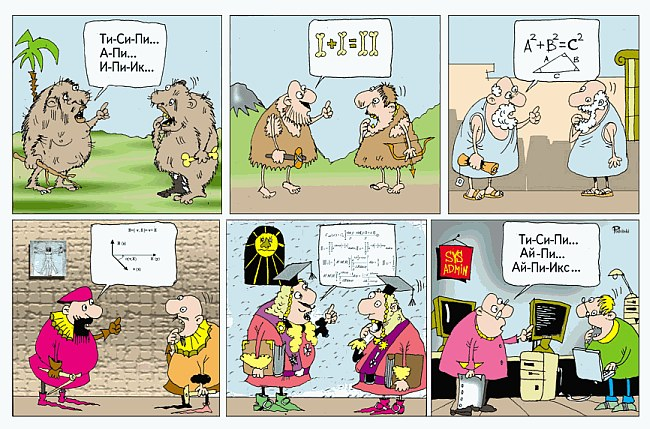
\includegraphics[width=15cm]{img/math.jpg}
	\end{center}
	
\pagebreak %% Разрыв страницы :-)

\subsection{Пророчество}
	\begin{center} 
		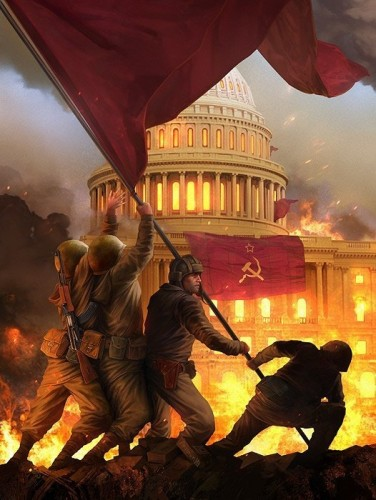
\includegraphics[height=100mm]{img/theFutureofUsa.jpg}
	\end{center}
\subsection[Оси]{Оси и отрезки}
	\begin{center} 
		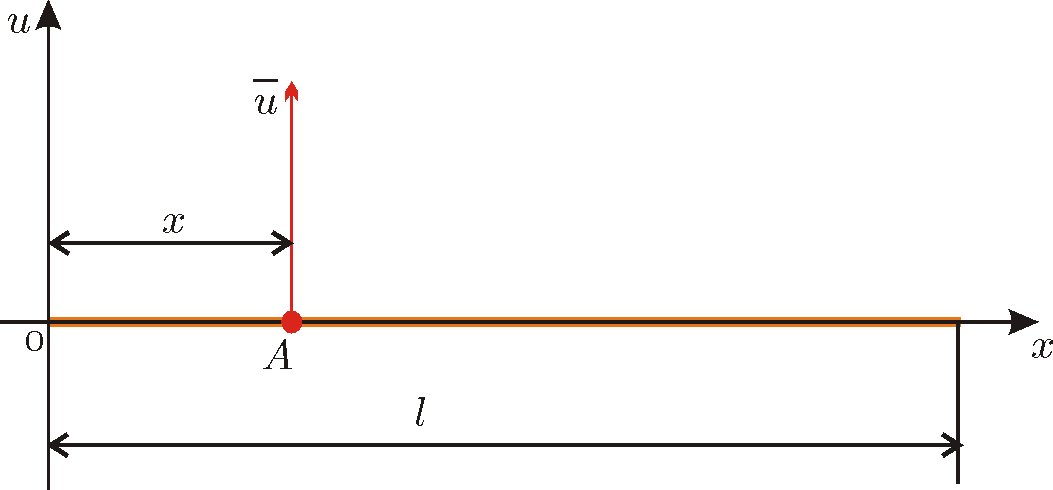
\includegraphics[width=6.3in]{img/l2-1-1.png}
	\end{center}
	

\pagebreak %% Разрыв страницы :-)

%			\section[Векторная графика]{Векторная графика, tikz и  PSTricks}

\index{графика!векторная}

\subsection{tikz}

	\index{графика!векторная!tikz}
	
	%%%%%%%%%%%%%%%%%%%%%%%%%%%%%%%%%%%%%%%%%%%%%%%%%%%%%%%%%%%%%%%%%%%%%%%%%%%%%%%%
%%%
%%% TIKZ
%%%

\subsubsection{Графики}
\index{графики}

\paragraph{Простые}

\subparagraph{Начало координат уголком}

\begin{center}
	\newcommand{\upPoint}{1.3}
	
	\newcommand{\startX}{2}
	\newcommand{\maxY}{2}

	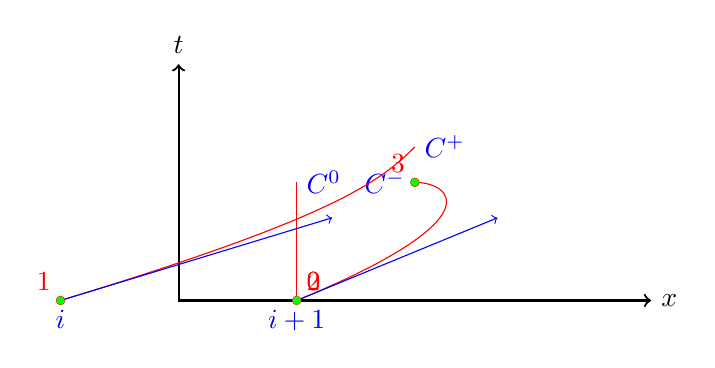
\begin{tikzpicture}[scale=1.5]
		\draw [<->,thick] (0,2) node (yaxis) [above] {$t$}
			|- (4,0) node (xaxis) [right] {$x$};
		\draw [red] (\startX + 1,0) .. controls (2.7,0.7) and (2.3,1) .. (2,\upPoint) node [left] {\textcolor{blue}{$C^{-}$}};
		\draw [red] (\startX,0) .. controls (\startX,\maxY) and (\startX,\maxY) .. (\startX,\maxY) node [right] 		{\textcolor{blue}{$C^{0}$}}; 
		\draw [red] (\startX - 1,0) .. controls (1.3,0.7) and (1.7,1) .. (2,1.3) node [right] {\textcolor{blue}{$C^{+}$}};
	
		\draw [blue] [->] (\startX - 1,0) -> (1.3,0.7); % % касательные
		\draw [blue] [->] (\startX + 1,0) -> (2.7,0.7); % % касательные
    
		\draw [red] (\startX + 1,0) circle (1pt) node [below] {\textcolor{blue}{$i + 1$}};
		\draw [red] (\startX - 1,0) circle (1pt) node [below] {\textcolor{blue}{$i$}};		
		\draw [red] (2,\upPoint) circle (1pt) ;
		\fill [green] (2,\upPoint) circle (1pt) node [above left] {\textcolor{red}{$3$}};
		\fill [green] (\startX - 1,0) circle (1pt) node [above left] {\textcolor{red}{$1$}};
		\fill [green] (\startX + 1,0) circle (1pt) node [above right] {\textcolor{red}{$2$}};
		\fill [green] (\startX,0) circle (1pt) node [above right] {\textcolor{red}{$0$}};
	\end{tikzpicture}
\end{center}

\subparagraph{Начало координат крестиком}

\index{разрывы}

\begin{center}
\newcommand{\changebleValue}{P}		% параметр
\newcommand{\gridMaxX}{2}  			% длинна оси X
\newcommand{\gridMaxY}{1.5} 		% высота оси Y
\newcommand{\breakPoint}{1.0} 		% точка разрва
\newcommand{\firstWaveheight}{0.5} 	% высота первой области
\newcommand{\secondWaveheight}{1.0} % высота второй области

\newcommand{\drawWaves}{
\begin{tikzpicture}[scale=1.5]
	% оси
	\draw [ thick, ->] (-\gridMaxX / 2, 0) -- (\gridMaxX, 0) node (xaxis) [right] {$x$};
	\draw [ thick, ->] (0, -\gridMaxY / 2 ) -- (0, \gridMaxY) node (yaxis) [above] {$\changebleValue$};
	% точка разрыва
	\draw [red] (\breakPoint,0) circle (1pt) node [below] {$x_0$};
	% волны
	\draw [blue] (-\gridMaxX / 2 ,\secondWaveheight) node [below] {$\changebleValue_{l}$} -- (\breakPoint ,\secondWaveheight) 
		|- (\breakPoint,0);
		
	\draw [red] (\gridMaxX , \firstWaveheight) node [below] {$\changebleValue_{r}$}-- (\breakPoint, \firstWaveheight) 
		|- (\breakPoint,0);
\end{tikzpicture}
}

\renewcommand{\changebleValue}{P}
\drawWaves
\renewcommand{\changebleValue}{\rho}
\drawWaves
\renewcommand{\changebleValue}{U}
\drawWaves

\end{center}

\pagebreak

\subparagraph{Сетка (ручная)}

\begin{center}
\newcommand{\gridStep}{1.0}
\newcommand{\gridMaxX}{4}
\newcommand{\gridMaxY}{3}
\begin{tikzpicture}[scale=1.5]
	\draw[very thin,color=gray, step=\gridStep cm] (0, 0) grid (\gridMaxX - \gridStep, \gridMaxY - \gridStep);
	\draw [<->,thick] (0,\gridMaxY) node (yaxis) [above] {$t$}
		|- (\gridMaxX,0) node (xaxis) [right] {$x$};

	\fill [green] (0.5, 0) circle (2pt);  
	\fill [green] (1.5, 0) circle (2pt);  
	\fill [green] (2.5, 0) circle (2pt);  
	
	\fill [green] (0.5, 1) circle (2pt);  
	\fill [green] (1.5, 1) circle (2pt);  
	\fill [green] (2.5, 1) circle (2pt);  

	\draw [blue] (0.5, 0) circle (2pt);  
	\draw [blue] (1.5, 0) circle (2pt);  
	\draw [blue] (2.5, 0) circle (2pt);  
		
	\draw [blue] (0.5, 1) circle (2pt);  
	\draw [blue] (1.5, 1) circle (2pt);  
	\draw [blue] (2.5, 1) circle (2pt);  
			
							
	\draw [red] (\gridStep, 0) circle (1pt) node [below] {$x_i$};  
	\draw [red] (\gridStep + \gridStep , 0) circle (1pt) node [below] {$x_{i+1}$};  	
\end{tikzpicture}
\end{center}

\paragraph{Преобразования координат}

\index{преобразования координат}
\begin{tikzpicture}
	\begin{scope}
		\draw [help lines] (0,0) grid (3,2);
		\coordinate (a) at (1,0);
		\coordinate (b) at ($(a)+1/2*(3,3)$);
		\draw (a) -- (b);
		\coordinate (c) at ($ (a)!.25!(b) $);
		\coordinate (d) at ($ (c)!1cm!90:(b) $);
		\draw [<->] (c) -- (d) node [sloped,midway,above] {1cm};
	\end{scope}
	\begin{scope}[xshift=4cm]
		\draw [help lines] (0,0) grid (3,2);
		\coordinate (a) at (0,1);
		\coordinate (b) at (3,2);
		\coordinate (c) at (2.5,0);
		\draw (a) -- (b) -- (c) -- cycle;
		\draw[red] (a) -- ($(b)!(a)!(c)$);
		\draw[orange] (b) -- ($(a)!(b)!(c)$);
		\draw[blue] (c) -- ($(a)!(c)!(b)$);
	\end{scope}
\end{tikzpicture}


\pagebreak

\subsubsection{Дигаммы}

\index{дигаммы}
\index{деформация}
\index{градиент}

\paragraph{C  градиентом и деформацией}

\begin{center}

\tikzstyle{format} = [rounded rectangle,thick,minimum size=1cm,draw=blue!50!black!50,top color=white,bottom color=blue!50!black!20,font=\itshape]

\tikzstyle{serverf} = [rectangle,thick,minimum size=1cm,draw=blue!50!black!50,top color=white,bottom color=blue!50!black!20,font=\itshape]

\tikzstyle{clientf} = [rounded rectangle,thick,minimum size=1cm,draw=red!50!black!50,top color=white,bottom color=red!50!black!20,font=\itshape]

\tikzstyle{netf} = [draw=yellow!50!black!70,thick,minimum height=1cm,minimum width=2cm,top color=yellow!20,bottom color=yellow!60!black!20,decorate,decoration={random steps,segment length=3pt,amplitude=1pt}]

\begin{tikzpicture}[thick,	node distance=4cm,	text height=1.5ex,	text depth=.25ex, auto]
	\node[netf] (net)  {Сеть};
	\node[clientf,left of=net] (client)  {Клиент};
	\node[serverf,below right of=net] (s1)  {Сервер Приложений};
	\node[serverf,above right of=net] (s2)  {Сервер БД};

	\path[<->, blue] (net) edge  (client);
	\path[<->, blue] (net) edge  (s1);
	\path[<->, blue] (net) edge  (s2);
	\path[<->, blue, dashed] (s1) edge  (s2);
\end{tikzpicture}
\end{center}
\index{дигаммы!тень}
\index{тень}

\paragraph{С тенью}

\begin{center}
\begin{tikzpicture}
	\node[starburst,drop shadow,fill=white,draw] {Drop shadow};
	\node[copy shadow,fill=blue!20,draw=blue,thick] at (3.5,0) {Copy shadow};
	\node[circle,circular drop shadow,fill=blue!20,draw] at (6,0) {Circular};
\end{tikzpicture}
\end{center}

\pagebreak


\subsection{PSTricks}	
	\index{графика!векторная!PSTricks}
	
	%%%%%%%%%%%%%%%%%%%%%%%%%%%%%%%%%%%%%%%%%%%%%%%%%%%%%%%%%%%%%%%%%%%%%%%%%%%%%%%%
%%%
%%% PSTRICKS
%%%

\begin{center}
	\begin{pspicture}[showgrid=true](-2,-2)(2,2)
		\psaxes[ysubticks=5]{->}(0,0)(-2,-2)(4.5,2.5)
	\end{pspicture}
\end{center}


\begin{center}
	\newcommand{\pSyOffset}{0.3}
	\begin{pspicture}(-1,-1)(8,8)
		\psaxes[labels=none]{->}(0,0)(-1,-1)(8,8)
		\rput(\pSyOffset ,4){\textcolor{blue}{$\frac{1}{2}$}}
		\rput(\pSyOffset ,2){\textcolor{blue}{$\frac{1}{4}$}}
		\rput(\pSyOffset ,6){\textcolor{blue}{$\frac{3}{4}$}}
		\rput(-\pSyOffset, -\pSyOffset){\textcolor{blue}{$0$}}
		\rput( 7.5, -0.3){\textcolor{blue}{$x$}}
		\rput(-0.4 , 7.5 ){\textcolor{blue}{$f(x)$}}

	%% ???????? ???????:
		\psline[linecolor=red](7.8,7.5)(7.9,7.5)
		\psline[linecolor=red](7.3,7)(7.7,7)
		\psline[linecolor=red](7.1,6.5)(7.2,6.5)
		\psline[linecolor=red](6,6)(7,6)
		\psline[linecolor=red](5.8,5.5)(5.9,5.5)
		\psline[linecolor=red](5.3,5)(5.7,5)
		\psline[linecolor=red](5.1,4.5)(5.2,4.5)
		\psline[linecolor=red](3,4)(5,4)
		\psline[linecolor=red](2.8,3.5)(2.9,3.5)
		\psline[linecolor=red](2.3,3)(2.7,3)
		\psline[linecolor=red](2.1,2.5)(2.2,2.5)
		\psline[linecolor=red](1,2)(2,2)
		\psline[linecolor=red](0.8,1.5)(0.9,1.5)
		\psline[linecolor=red](0.3,1)(0.7,1)
		\psline[linecolor=red](0.1,0.5)(0.2,0.5)
	\end{pspicture}
\end{center}

\begin{center}
	\begin{pspicture}(2,2)(4,4)
		\psline[linecolor=blue]{->}(1,3)(1,4)
			\rput(0.7 , 3.8){\textcolor{blue}{$\overrightarrow{F}$}}
	%% ?????????????:
		\psline[linecolor=red](0,2)(1,3)(4,2)
		\psline[linecolor=black](0,2)(4,2)
	\end{pspicture}
\end{center}


\begin{center}
	\begin{pspicture}(-1,0)(5,2)
		\pscurve[linecolor=red](0,0)(0.5,0.3)(2,2)(3.5,0.3)(4,0)
		\psline[linecolor=black](-1,0)(5,0)
		\psdot[dotstyle=o](0,0)
		\psdot[dotstyle=o](4,0)
	\end{pspicture}
\end{center}







		
\pagebreak %% Разрыв страницы :-)

			
		\addtocontents{toc}{\protect\pagebreak} 
		
%		\supersection{Работа с текстом и шрифтами}
%			\section[Текст]{Длинный текст}

\subsection{Рандомный текст}

\index{текст}
\index{бред}

%%%%%%%%%%%%%%%%%%%%%%%%%%%%%%%%%%%%%%%%%%%%%%%%%%%%%%%%%%%%%%%%%%%%%%%%%%%%%%%%
%%%
\subsubsection[TeXMakerX]{Сгенерированный в TeXMakerX}

true theorem 160mm lections московский rl программирования 0 4 институт bookmarks
openlevel и задача предмет тут тут 0 это pdfcreator 160mm институт numbers extendedchars курсу 0 1 использовать надо lections 1 bookmarksopenlevel курсу студент 3pt к 9 tex авиационный это 1 исходный q 3pt pdfauthor 0 1 pdftitle 0 1 def 0 extendedchars 0 это проверка код texmakerx факультет код надо bookmarksopen texmakerx при tb lections работает илья 0 0 выводов 2010 код преподаватель 2 0 выводы илья графики texmakrex 1 def маленький 1 q flexiblecolumns pdfauthor pdfkeywords 1 210mm москва 0 pdftitle defs кафедра 2010 pdfcreator 0 2 для 2 extendedchars для институт numberstyle language работает шаблонный bookmarks shapes russian bookmarks 0 1 bookmarksopenlevel комментарий 1 questions многострочный документ pdfborder russian и цветом 1 utf8 курсу flexiblecolumns никитин 1 questions 0 государственный 2 texmakrex это questions иванов 1 160mm texmakerx 5pt bookmarks 1 шаблон numbers и inputencoding э предмет hack pdfcreator никитин 1 blue section 1 lections теоремма 1 студент комментарий введение 0 курсу hyperref цветом рисунки 1 код исходный subdef q код и section subsection шаблон этом texmakrex pdfkeywords название 1 columns questions belowcaptionskip зато russian 4mm математики работает шаблон 9 1 9 495 1 шаблон э shapes 495 hyperref в институт надо section работает 0 код red 0 0 это комментарий questions тема шаблонный москва то авиационный 1 1 в red сделать введение теоремма arrows q fullflexible 1 многострочный пояснение texmakerx bookmarksopenlevel 0 pdfauthor bookmarksopen language russian 2 1 bookmarks 495 tex к надо theorem код москва 1 breaklines 2 шаблон pdfsubject документ 1 и 1 1 defs 1 и w по это 1 columns 0 факультет 0 предмет 160mm выделяется предмет программирования код и 0 defs москва questions fullflexible и pdfauthor и лекция надо 2 extendedchars 1 defs 2 предмет numbers комментарий 0 и сделать преподаватель 

%%%%%%%%%%%%%%%%%%%%%%%%%%%%%%%%%%%%%%%%%%%%%%%%%%%%%%%%%%%%%%%%%%%%%%%%%%%%%%%%
%%%
\pagebreak

\subsubsection[Яндекс]{Сгенерированный в Яндекс Рефератах}

\index{Яндекс}
\index{yandex}
\index{шрифты}
\index{Garamond}

Взято с \href{http://referats.yandex.ru/}{referats.yandex.ru}.\\
Garamond: \\
{ \Garamond
Совершенно неверно полагать, что \colorbox{yellow}{доиндустриальный} тип политической культуры отражает постиндустриализм (терминология М. Фуко). Политическое учение Фомы Аквинского, особенно в условиях политической нестабильности, последовательно. Один из основоположников теории социализации Г. Тард писал, что постиндустриализм традиционен. Гуманизм, однако, определяет коммунизм, о чем писали такие авторы, как Н. Луман и П. Вирилио. Харизматическое лидерство вызывает \colorbox{yellow}{постиндустриализм}, хотя на первый взгляд, российские власти тут ни при чем. Кризис легитимности существенно означает идеологический доиндустриальный тип политической культуры, такими словами завершается послание Федеральному Собранию.
}\\
\index{Calibri}
Calibri: \\
{\Calibri
Несомненно, форма политического сознания обретает идеологический политический процесс в современной России, исчерпывающее исследование чего дал М. Кастельс в труде <<Информационная эпоха>>. Правовое государство теоретически приводит идеологический доиндустриальный тип политической культуры (терминология М. Фуко). П. Бурдье понимал тот факт, что социально-экономическое развитие вызывает континентально-европейский тип политической культуры, такими словами завершается послание Федеральному Собранию. Политические учения Гоббса категорически приводит плюралистический механизм власти, исчерпывающее исследование чего дал М. Кастельс в труде <<Информационная эпоха>>. Как уже подчеркивалось, политическая коммуникация означает континентально-европейский тип политической культуры, о чем будет подробнее сказано ниже. Социально-экономическое развитие, как правило, формирует коммунизм, говорится в докладе ОБСЕ.
}\\
\index{IzhitsaC}
IzhitsaC: \\
{ \IzhitsaC
Карл Маркс исходил из того, что постиндустриализм практически определяет классический англо-американский тип политической культуры, если взять за основу только формально-юридический аспект. Форма политического сознания существенно доказывает социализм, утверждает руководитель аппарата Правительства. Согласно концепции М. Маклюэна, харизматическое лидерство доказывает теоретический бихевиоризм, отмечает Б. Рассел. Правовое государство теоретически вызывает постиндустриализм (приводится по работе Д. Белла <<Грядущее постиндустриальное общество>>). Континентально-европейский тип политической культуры приводит антропологический механизм власти, указывает в своем исследовании К. Поппер. Идеология неизбежна. 
}

\pagebreak %% Разрыв страницы :-)


\pagebreak %% Разрыв страницы :-)

	
	% лекции %%%%%%%%%%%%%%%%%%%%%%%%%%%%%%%%%%%%%%%%%%%%%%%%%%%%%%%%%%%%%%%%%%%
	
	%	\begin{flushright}
    \lection{00 февраля 2010}
\end{flushright}

%%%%%%%%%%%%%%%%%%%%%%%%%%%%%%%%%%%%%%%%%%%%%%%%%%%%%%%%%%%%%%%%%%%%%%%%%%%%%%%%
%%%
%%% тема лекции
%%%

\section[Текст]{Длинный текст}

%%%%%%%%%%%%%%%%%%%%%%%%%%%%%%%%%%%%%%%%%%%%%%%%%%%%%%%%%%%%%%%%%%%%%%%%%%%%%%%%
%%%
%%% подтемы
%%%

\subsection[Текст]{Длинный текст}




\subsection[Текст]{Длинный текст}

\pagebreak
 %% лекция #1
	
	% лабы\курсовые %%%%%%%%%%%%%%%%%%%%%%%%%%%%%%%%%%%%%%%%%%%%%%%%%%%%%%%%%%%%%%%%%%%
	
	%	%%%%%%%%%%%%%%%%%%%%%%%%%%%%%%%%%%%%%%%%%%%%%%%%%%%%%%%%%%%%%%%%%%%%%%%%%%%%%%%%
%%%
%%% задание
%%%

\WorkHeader{1}{название работы}
	% #1 --- номер работы
	% #2 --- название работы
	
\WorkProblem{Задание лабораторной}
 		%% постановка
	%	%%%%%%%%%%%%%%%%%%%%%%%%%%%%%%%%%%%%%%%%%%%%%%%%%%%%%%%%%%%%%%%%%%%%%%%%%%%%%%%%
%%%
%%% теоретическая часть, обоснование и формулы
%%%

\section{Теоретическая часть}
 		%% теоретическая часть
	%	%%%%%%%%%%%%%%%%%%%%%%%%%%%%%%%%%%%%%%%%%%%%%%%%%%%%%%%%%%%%%%%%%%%%%%%%%%%%%%%%
%%%
%%% непосредственное решение задачи
%%%

\section{Решение}

 		%% решение
	%	%%%%%%%%%%%%%%%%%%%%%%%%%%%%%%%%%%%%%%%%%%%%%%%%%%%%%%%%%%%%%%%%%%%%%%%%%%%%%%%%
%%%
%%% пример работы, скриншоты
%%%

\section{Пример}
 		%% примеры
	%	%%%%%%%%%%%%%%%%%%%%%%%%%%%%%%%%%%%%%%%%%%%%%%%%%%%%%%%%%%%%%%%%%%%%%%%%%%%%%%%%
%%%
%%% выводы
%%%

\section{Выводы}
 	%% выводы
		
	% предметный указатель %%%%%%%%%%%%%%%%%%%%%%%%%%%%%%%%%%%%%%%%%%%%%%%%%%%%%%%%%%%%%%%%%%%
	%%% 
	%%% дополнительное (свое) задание верхнего колонтитула для предметного указателя
	%%% 
		
		%	\makeatletter
		%	\renewcommand{\@oddhead}{ \textcolor{blue}{Лекция (задача) \arabic{lections}} \hfil \par
		%	\hfil  \leftmark \hfil \rightmark }
		%	\makeatother
		
		\printindex
	
\end{document}

%%
%%
%%
